\clearpage
\section{\HellingerCaseTitle: Hellinger-to-TV upper bound}
\label{app:upper-proof}

\textcolor{red}{We prove the finite TV guarantee for the sampler in
Appendix~\ref{app:algorithm}; \cref{app:upper-proof-overview} gives the proof map.
Screen certification, peeling, and resource counts support both accuracy
cases via \eqref{app:eq:kl-oracle-inclusion}. The error analysis here proves
\HellingerCase; Appendix~\ref{app:kl-extension} proves \KLCase.
Appendix~\ref{app:benchmark-specializations} specializes both to
\cref{main:thm:upper-curve}.}
\ifincludeexponents
Its subsequent corollaries give joint-limit rates.
\fi
\ifincludeexponents
Independent-signal rates are collected in
Appendix~\ref{app:independent-signal}.
\fi

\subsection{Finite upper bound}
\label{app:results-upper}

The finite theorem uses the standard preprocessing floor of
Appendix~\ref{app:algorithm-preprocessing}; its query bound uses the realized
vocabulary-bank sizes $\BankSize{i}=|\TokenBank{i}|$.
Together with \cref{app:lem:benchmark-feasibility}, it yields
\HellingerCase\ of \cref{main:thm:upper-curve} through
\cref{app:cor:fixed-accuracy-main}.

\begin{theorem}[\HellingerCaseTitle: finite randomized Hellinger-to-TV upper bound]
\label{app:thm:finite-upper}
We work in \HellingerCase, with the oracle condition of
Assumption~\ref{app:ass:oracle-accuracy}.
Fix $N\ge10$ and the objects of Appendix~\ref{app:setup}.  Let
$\RandomizedPackedSampler$ be Algorithm~\ref{app:alg:complete-sampler} with
the standard zero-query draft of \eqref{app:eq:standard-draft} and
$\ScreenFailureBudget\in(0,1)$.  Suppose preprocessing is feasible and
\begin{equation}
 \ScreenResolution<\EdgeSignal.
 \label{app:eq:finite-screen-separation}
\end{equation}
Here $\RandomColorCount,\RandomColoringCount$ are defined in
\eqref{app:eq:random-color-parameters}, and
$\ScreenCallCap,\HardRoundCap$ in
\eqref{app:eq:screen-call-and-round-caps}; $\ScreenColumnCount$ is
$\MaxBankSize+1$ when $\MaxBankSize\ge1$ and zero when $\MaxBankSize=0$, as in
\eqref{app:eq:screen-column-count}.
Then, for every admissible frozen oracle, pathwise over the random colors
and product-commit draws,
\begin{align}
 \CounterfactualQueries
 &\le \ScreenColumnCount\ScreenCallCap\RandomColoringCount
       \RandomColorCount(\RandomColorCount+\ChunkCount),
 \label{app:eq:finite-upper-Q}\\
 \CommitRounds
 &\le\HardRoundCap.
 \label{app:eq:finite-upper-R}
\end{align}
Moreover,
\begin{equation}
 \SeedRisk(\RandomizedPackedSampler;\TargetLaw,\FrozenOracle)
 \le
 \OracleRadius+\ScreenFailureBudget
 \quad\text{for every }
 \FrozenOracle\in\OracleClass(\TargetLaw;\OracleRadius).
 \label{app:eq:finite-upper-seed-risk}
\end{equation}
Consequently,
\begin{equation}
 \RobustRisk(\RandomizedPackedSampler;\TargetLaw)
 \le
 \OracleRadius+\ScreenFailureBudget.
 \label{app:eq:finite-upper-risk}
\end{equation}
In particular, if $\OracleRadius>0$ and
\begin{equation}
 \ScreenFailureBudget:=\frac{\OracleRadius}{2},
 \label{app:eq:finite-failure-budget-choice}
\end{equation}
then
$\RobustRisk(\RandomizedPackedSampler;\TargetLaw)\le3\OracleRadius/2$.
If the distinguished all-mask readout is charged, then
$\ReportedQueries=\CounterfactualQueries+1$ by
\eqref{app:eq:reported-query-count}.  Thus the bound for
$\ReportedQueries$ is the right-hand side of
\eqref{app:eq:finite-upper-Q} plus one; $\CounterfactualQueries$ still
excludes that readout.
Including that initial stage, the adaptive oracle depth is at most
$\OracleDepth\le1+\CommitRounds+\ScreenCallCap$.
\end{theorem}

\subsection{\texorpdfstring{\textcolor{red}{Proof overview}}{Proof overview}}
\label{app:upper-proof-overview}

{\color{red}
The proof turns local screen certificates into safe parallel commits:
accurate low-degree rows make peeling contract the high-degree core, after
which the remaining forest is known and its components can be sampled in
parallel.  We then bound resources and output error separately.
\Cref{app:tab:upper-proof-map} follows this chain under the finite hypotheses
above.  The structural certificates hold when every reached screen succeeds;
the resource caps hold on every path.  The same construction supports both
accuracy cases, with different output-error arguments.

\begin{table}[H]
\centering
\small
\color{red}
\setlength{\tabcolsep}{4pt}
\begin{tabularx}{\linewidth}{@{}>{\raggedright\arraybackslash}p{0.17\linewidth}
  >{\raggedright\arraybackslash}X
  >{\raggedright\arraybackslash}p{0.14\linewidth}
  >{\raggedright\arraybackslash}p{0.19\linewidth}@{}}
\toprule
Proof task & Key argument and conclusion & Algorithm steps & References \\
\midrule
\textbf{Certify the vocabulary banks}
& Preprocessing gives a nonempty complement of $\TokenBank{i}$, whose
tokens have true marginal mass below $\TailThreshold$, certifying the
tail representative.  Under the standard floor, (RF) bounds
$\BankSize{i}\le(4\FrequencyConstant/\TailThreshold)^{1/\RankTailExponent}$.
& \AlgoBlockRef{preprocess}
& \cref{app:lem:preprocessing-certificates} \\
\addlinespace
\textbf{Recover low-degree neighborhoods}
& Separating colors reduce packed probes to one-source comparisons at a
fixed boundary.  RT--UEN and the screening margin make their votes correct;
fresh-color majorities give
$\ScreenRow{j}=\mathcal N_{\ResidualForest}(j)$ for degree at most
$\DegreeCutoff$, except on reached-screen failures of total probability
at most $\ScreenFailureBudget$.
& \AlgoBlockRef{draft}--\AlgoBlockRef{screen};
\AlgoBlockRef{chunks}--\AlgoBlockRef{aggregate}
& \cref{app:lem:residual-markov,app:lem:random-screen-success,app:lem:fixed-draft-rows};
\AppLowDegreeScreenRef \\
\addlinespace
\textbf{Peel the high-degree core}
& Let $\HighDegreeCount{k}$ count vertices of degree above $\DegreeCutoff$
before phase $k$.  On successful paths, the forest degree sum gives
$\HighDegreeCount{k+1}\le(4/\DegreeCutoff)\HighDegreeCount{k}$.
Either stopping test leaves maximum degree at most $\DegreeCutoff$,
certifying the true residual forest.
& \AlgoBlockRef{peel}--\AlgoBlockRef{terminal}
& \cref{app:lem:successful-path-structure} \\
\addlinespace
\textbf{Complete safe parallel sampling}
& Singleton peels and one centroid per true residual component are safe.
Exact-row products then equal joint batch conditionals.  Centroid deletion
halves component sizes, giving logarithmically many terminal rounds on
successful paths.
& \AlgoBlockRef{peel}, \AlgoBlockRef{centroid}
& \cref{app:lem:residual-markov,app:lem:upper-resources,app:lem:exact-hybrid} \\
\addlinespace
\textbf{Bound all-path resources}
& Count screen loops for $\CounterfactualQueries$, and peel and centroid
commits for rounds.  \AlgoGuardRef\ caps rounds even on failed-screen paths.
Each screen is one parallel stage:
$\OracleDepth\le1+\CommitRounds+\ScreenCallCap$.
$\CounterfactualQueries$ excludes preprocessing and commits.
& All: \AlgoBlockRef{preprocess}--\AlgoBlockRef{centroid}, plus \AlgoGuardRef
& \cref{app:lem:upper-resources} \\
\addlinespace
\textbf{\HellingerCaseTitle: bound output TV}
& Each coordinate is committed once, so adaptive Hellinger composition
bounds an analysis-only safe rule's oracle error.  Coupling to that rule adds at most
$\ScreenFailureBudget$, giving seed-averaged TV at most
$\OracleRadius+\ScreenFailureBudget$.
& All: \AlgoBlockRef{preprocess}--\AlgoBlockRef{centroid}; output-law analysis
& \cref{app:lem:exact-hybrid,app:lem:adaptive-hellinger-upper,app:lem:safe-controller-comparison};
\cref{app:thm:finite-upper} \\
\addlinespace
\textbf{\KLCaseTitle: bound output KL}
& With forward row KL at most $\KLRowBudget$, the joint-reference identity
separates row error from batch total correlation.  The latter vanishes
on successful reference paths, giving seed-averaged KL at most
$N\KLRowBudget+N\log\VocabSize\,\ScreenFailureBudget$.
& All: \AlgoBlockRef{preprocess}--\AlgoBlockRef{centroid}; output-law analysis
& \cref{app:lem:adaptive-joint-kl,app:thm:finite-kl-upper} \\
\addlinespace
\textbf{Recover the main theorem}
& Verify preprocessing feasibility and screen separation for the main-text
scaling, then specialize the finite bounds and choose the degree cutoff.
Both cases yield \cref{main:thm:upper-curve}.
& All: \AlgoBlockRef{preprocess}--\AlgoBlockRef{centroid}; parameter choices
& \cref{app:lem:benchmark-feasibility,app:cor:fixed-accuracy-main} \\
\bottomrule
\end{tabularx}
\caption{Proof steps for the upper bound.  Step labels link to
Algorithms~\ref{app:alg:complete-sampler}--\ref{app:alg:packed-screen}.}
\label{app:tab:upper-proof-map}
\end{table}

Two distinctions guide the proof:
\begin{itemize}
\item High-degree rows need only satisfy the size cap
$|\ScreenRow{j}|\le\DegreeCutoff$.  Accurate low-degree rows suffice to
force contraction, even when high-degree rows are incorrect.
\item For \HellingerCase, an analysis-only safe rule switches to singleton
completion at the first failed screen (and before any cap fallback).
We compare its full output law with the implemented sampler's law;
no conditioning of the output on screen success is needed.
\end{itemize}
Combining these bounds gives \cref{app:eq:randomized-upper-TV-proof}:
\[
 \mathbb E_{\ControllerSeed}
 \dTV\bigl(\TargetLaw,
            \SamplerOutputLaw{\ControllerSeed}{\FrozenOracle}\bigr)
 \le
 \underbrace{\OracleRadius}_{\text{oracle error at commits}}
 +\underbrace{\ScreenFailureBudget}_{\text{failed-screen coupling}}.
\]
\par}

\subsection{\texorpdfstring{\textcolor{red}{Steps 1--3: }}{Steps 1--3: }Preprocessing and exact low-degree certification}
\label{app:upper-proof-screen}

We first establish the residual Markov and tail certificates, then prove the
fresh-color success bound and the low-degree screen contract.
\textcolor{red}{These certify the vocabulary banks from
\AlgoBlockNamedRef{preprocess}, the fresh colors from
\AlgoBlockNamedRef{draft}, and the rows returned by
\AlgoBlockNamedRef{screen}.}

The next lemma derives the residual Markov property from
\cref{main:eq:forest-factorization}.
Recall from \eqref{app:eq:history} that
$\ResidualPositions=\PositionSet\setminus G$ and
$\ResidualForest=\TargetForest[\ResidualPositions]$.
\textcolor{red}{Its row identity is used in \AlgoBlockNamedRef{probes},
and its component independence justifies \AlgoBlockNamedRef{centroid}.}

\begin{lemma}[Residual Markov property]
\label{app:lem:residual-markov}
Fix a history $\History=(G,x_G)$.  Conditional on $X_G=x_G$, the variables in
distinct connected components of $\ResidualForest$ are independent.  Moreover,
fix $j\in\ResidualPositions$ and the values of all residual neighbors of $j$.
The exact conditional row of $X_j$ is unchanged if any residual nonneighbor is
revealed, masked, changed, or marginalized.
\end{lemma}

\begin{proof}

\emph{1. Factor the conditional law over residual components.}
Recall the forest factorization \eqref{app:eq:S0}:
$\TargetLaw(x)=\prod_{u\in\TargetRoots}\PosMarginal{u}(x_u)
 \prod_{j\notin\TargetRoots}\EndpointKernel{\ParentOf{j}}{j}
 (x_j\mid x_{\ParentOf{j}})$.
Here $\TargetRoots$ and $\ParentOf{\cdot}$ are the original reference roots
and parent map.  Substitute the fixed committed values $x_G$.
For each connected component $T$ of $\ResidualForest$, identified with
its vertex set, define
\[
\begin{aligned}
 g_T(x_T):={}&
 \prod_{u\in\TargetRoots\cap T}\PosMarginal{u}(x_u)
 &&\text{roots in }T\\
 &{}\times
 \prod_{\substack{j\in T\setminus\TargetRoots\\\ParentOf{j}\in T}}
 \EndpointKernel{\ParentOf{j}}{j}(x_j\mid x_{\ParentOf{j}})
 &&\text{edges within }T\\
 &{}\times
 \prod_{\substack{j\in T\setminus\TargetRoots\\\ParentOf{j}\in G}}
 \EndpointKernel{\ParentOf{j}}{j}(x_j\mid x_{\ParentOf{j}})
 &&\text{edges }G\to T\\
 &{}\times
 \prod_{\substack{j\in G\setminus\TargetRoots\\\ParentOf{j}\in T}}
 \EndpointKernel{\ParentOf{j}}{j}(x_j\mid x_{\ParentOf{j}})
 &&\text{edges }T\to G.
\end{aligned}
\]
The fixed $x_G$ dependence is suppressed in $g_T$.
In particular, the last product retains factors for committed children of
vertices in $T$: their parent values still vary with $x_T$.
Every edge with a residual endpoint is either internal to one such $T$ or
crosses between $T$ and $G$; no edge joins distinct residual components.
Thus, with products over $T$ ranging over these connected components,
\[
 \TargetLaw(x_G,x_{\ResidualPositions})
 =
 \left[
 \prod_{u\in\TargetRoots\cap G}\PosMarginal{u}(x_u)
 \prod_{\substack{j\in G\setminus\TargetRoots\\\ParentOf{j}\in G}}
 \EndpointKernel{\ParentOf{j}}{j}(x_j\mid x_{\ParentOf{j}})
 \right]\prod_T g_T(x_T).
\]
The bracket is positive and depends only on $x_G$.
It therefore cancels when dividing this joint probability by
$\TargetLaw(X_G=x_G)
 =\sum_{z_{\ResidualPositions}}\TargetLaw(x_G,z_{\ResidualPositions})$.
Since the connected components partition $\ResidualPositions$,
finite distributivity gives
\[
 \sum_{x_{\ResidualPositions}}\prod_T g_T(x_T)
 =\prod_T\left(\sum_{x_T}g_T(x_T)\right).
\]
Consequently
\[
\begin{aligned}
 \TargetLaw(X_{\ResidualPositions}=x_{\ResidualPositions}\mid X_G=x_G)
 &=\frac{\prod_T g_T(x_T)}
         {\sum_{z_{\ResidualPositions}}\prod_T g_T(z_T)}\\
 &=\prod_T\frac{g_T(x_T)}{\sum_{z_T}g_T(z_T)}.
\end{aligned}
\]
All sums range over the vocabulary assignments on their indicated vertex
sets; their denominators are positive by strict positivity of the factors.
This proves conditional independence of the residual components.


\emph{2. Cancel all factors not incident to the readout.}
For the second claim, root the original connected component at $j$,
using (C0).
Every original neighbor $v$ of $j$ is observed: either $v\in G$, or its
value is fixed in the lemma.  Call this value $x_v$.  The factors involving
$X_j=a$ are exactly
\[
 \PosMarginal{j}(a)
 \prod_{v\in\mathcal N_{\TargetForest}(j)}
       \EndpointKernel{j}{v}(x_v\mid a).
\]
All other factors are independent of $a$ once these neighbor values are
fixed.  Revealing, changing, or summing out nonneighbors only changes a
multiplicative factor independent of $a$.  It cancels in the normalized row
\[
 \frac{\PosMarginal{j}(a)
       \prod_{v\in\mathcal N_{\TargetForest}(j)}
          \EndpointKernel{j}{v}(x_v\mid a)}
      {\sum_{b\in\Vocab}\PosMarginal{j}(b)
       \prod_{v\in\mathcal N_{\TargetForest}(j)}
          \EndpointKernel{j}{v}(x_v\mid b)}.
\]
Thus the history and fixed neighbor values determine the row.
\end{proof}

The next lemma certifies the omitted tokens for screening and, under (RF\textcolor{red}{; \cref{app:eq:RF}})
with the standard floor, bounds the number of source columns.

\paragraph{Intuition.}
The local vocabulary bank $\TokenBank{i}$ from \eqref{app:eq:local-bank}
includes every token whose true marginal mass exceeds $\TailThreshold$.  Conversely, under the standard floor, every included
token has true mass at least $\TailThreshold/2$.
The rank envelope then bounds how many such tokens exist:
\[
 \frac{\TailThreshold}{2}
 \le\FrequencyConstant(\BankSize{i}^{-\RankTailExponent}+\VocabSize^{-1}),
 \quad
 \FrequencyConstant\VocabSize^{-1}\le\frac{\TailThreshold}{4}
 \quad\Longrightarrow\quad
 \BankSize{i}\le(4\FrequencyConstant/\TailThreshold)^{1/\RankTailExponent}.
\]
This is an upper bound on bank size; (RF\textcolor{red}{; \cref{app:eq:RF}}) does not require the envelope to
be attained.  The complementary tokens can all be represented by one
certified tail token in the response test.

\begin{lemma}[Preprocessing certificates\textcolor{red}{; \AlgoBlockRef{preprocess}}]
\label{app:lem:preprocessing-certificates}
Suppose preprocessing in \cref{app:def:preprocessing} is feasible, and let
$\TailThreshold$ be the threshold it selects.  Every local vocabulary bank
$\TokenBank{i}$ has a nonempty complement in $\Vocab$, so each
$\TailRepresentative{i}$ is well-defined.  For every
$i\in\PositionSet$ and $a\in\Vocab$,
\begin{equation}
 \bigl|\PosMarginal{i}(a)-\NoisyMarginal{i}(a)\bigr|
 \le\RowTVError,
 \qquad
 a\notin\TokenBank{i}
 \Longrightarrow a\in\TailSet{i}{\TailThreshold}.
 \label{app:eq:proof-preprocessing-certificates}
\end{equation}
Under (RF\textcolor{red}{; \cref{app:eq:RF}}), the standard floor \eqref{app:eq:rate-threshold-floor}
additionally gives
\begin{equation}
 \BankSize{i}
 \le\left(\frac{4\FrequencyConstant}{\TailThreshold}\right)^{1/\RankTailExponent}
 \quad\text{for every }i.
 \label{app:eq:finite-bank-size-proof}
\end{equation}
\end{lemma}

\begin{proof}

\emph{1. Establish a nonempty vocabulary-bank complement.}
In \AlgoBlockNamedRef{preprocess}, preprocessing fixes
$\TailThreshold=\max\FeasibleThresholdGrid$ once from the
public parameters, before the all-mask submission; this threshold is reused
by every screen.
Since $\FrequencyConstant\ge1$, the standard floor satisfies
$\ThresholdFloor=4\max\{\RowTVError,\FrequencyConstant/\VocabSize\}
\ge2(\RowTVError+1/\VocabSize)$.
Together with $\TailThreshold\ge\ThresholdFloor$, this gives
\begin{equation}
 \TailThreshold-\RowTVError
 \ge\RowTVError+\frac2{\VocabSize}
 >\frac1{\VocabSize}
 \ge\min_{a\in\Vocab}\NoisyMarginal{i}(a).
 \label{app:eq:baseline-existence}
\end{equation}
Thus $\TokenBank{i}\ne\Vocab$, proving tail-representative existence.

\emph{2. Certify every omitted token using the row-TV bound.}
At the all-mask state, $\ExactRow{\AllMaskState}{i}=\PosMarginal{i}$ and
$\OracleRow{\AllMaskState}{i}=\NoisyMarginal{i}$.
Thus \eqref{app:eq:oracle-tv-radius} and the singleton-event bound for TV give,
for every $a\in\Vocab$,
\[
 \bigl|\PosMarginal{i}(a)-\NoisyMarginal{i}(a)\bigr|
 \le \sup_{A\subseteq\Vocab}
       \bigl|\PosMarginal{i}(A)-\NoisyMarginal{i}(A)\bigr|
 =\dTV(\PosMarginal{i},\NoisyMarginal{i})
 \le\RowTVError.
\]
This bounds both signs of the difference, whether or not $a$ belongs to
$\TokenBank{i}$.  For a token outside the vocabulary bank $\TokenBank{i}$,
definition \eqref{app:eq:local-bank} then gives
\begin{equation}
 a\notin\TokenBank{i}
 \quad\Longrightarrow\quad
 \PosMarginal{i}(a)
 \le\NoisyMarginal{i}(a)+\RowTVError<\TailThreshold.
 \label{app:eq:bank-complement-tail}
\end{equation}
This proves \eqref{app:eq:proof-preprocessing-certificates}, including the
tail certificate for $\TailRepresentative{i}$.


\emph{3. Apply (RF\textcolor{red}{; \cref{app:eq:RF}}) only for the bank-size estimate.}
For the vocabulary-bank size $\BankSize{i}=|\TokenBank{i}|$,
the standard floor gives
$\TailThreshold\ge\ThresholdFloor=\StandardThresholdFloor{\FrequencyConstant}$,
hence both $\TailThreshold\ge4\RowTVError$ and
$\TailThreshold\ge4\FrequencyConstant/\VocabSize$.
Every $a\in\TokenBank{i}$ therefore satisfies
\begin{equation}
 \PosMarginal{i}(a)
 \ge\NoisyMarginal{i}(a)-\RowTVError
 \ge\TailThreshold-2\RowTVError
 \ge\frac{\TailThreshold}{2}.
 \label{app:eq:bank-member-mass}
\end{equation}
If
$\BankSize{i}\ge1$, at least $\BankSize{i}$ tokens have exact mass at least
$\TailThreshold/2$; hence the exact rank-$\BankSize{i}$ mass has the same
lower bound.  Assumption (RF\textcolor{red}{; \cref{app:eq:RF}}) and
$\TailThreshold\ge4\FrequencyConstant/\VocabSize$ yield
\[
 \frac{\TailThreshold}{2}
 \le\FrequencyConstant
 \left(\BankSize{i}^{-\RankTailExponent}+\VocabSize^{-1}\right)
 \le\FrequencyConstant\BankSize{i}^{-\RankTailExponent}
    +\frac{\TailThreshold}{4}.
\]
Rearranging proves \eqref{app:eq:finite-bank-size-proof}.  The inequality is
trivial when $\BankSize{i}=0$.
\end{proof}

\paragraph{Screen-success event (analysis only).}
\textcolor{red}{The colors drawn in \AlgoBlockNamedRef{draft} determine
the following event for \AlgoBlockNamedRef{screen}.}
Fix a realized history $\History=(G,x_G)$.  For distinct
$i,j\in\ResidualPositions$ with
$d_{\ResidualForest}(j)\le\DegreeCutoff$, call $\tau$
\emph{$(i,j)$-separating} when
\begin{equation}
\begin{aligned}
 \ColorHash{\tau}{v}&\ne\ColorHash{\tau}{j}
   &&\text{for every }v\in\mathcal N_{\ResidualForest}(j),\\
 \ColorHash{\tau}{v}&\ne\ColorHash{\tau}{i}
   &&\text{for every }
   v\in\mathcal N_{\ResidualForest}(j)\setminus\{i\}.
\end{aligned}
\label{app:eq:pair-separating-coloring}
\end{equation}
The screen family is \emph{successful at $\History$}, denoted
$\ScreenSuccess{\History}$, if
\begin{equation}
 \left|
 \left\{\tau\in\ColoringIndexSet:
       \tau\text{ is $(i,j)$-separating}\right\}
 \right|>\frac{\ColoringCount}{2}
 \label{app:eq:screen-success-event}
\end{equation}
for every such ordered pair $(i,j)$.  This event is defined using the hidden
residual forest only for analysis; the implemented screen neither observes
nor tests it.  For every separating $\tau$, the two properties used by the
screen proof are
\begin{equation}
 \mathcal N_{\ResidualForest}(j)
 \cap\ColorClass{\tau}{\ColorHash{\tau}{j}}=\emptyset,
 \qquad
 \mathcal N_{\ResidualForest}(j)
 \cap\ColorClass{\tau}{\ColorHash{\tau}{i}}\subseteq\{i\}.
 \label{app:eq:pairwise-local-isolation}
\end{equation}
\begin{example}[Checking which colors separate a pair]
\label{ex:algorithm-separation-20260918}
Use the coloring drawn in \AlgoBlockRef{draft} from
\cref{ex:algorithm-submissions-20260918} and the forest in
\cref{ex:algorithm-peel-centroids-20260918}.  For the tested pair
$(i,j)=(1,10)$, the readout has neighbors
$\mathcal N_{\ResidualForest}(10)=\{1,11\}$.  The two tests in
\eqref{app:eq:pairwise-local-isolation} are therefore
\[
 \{1,11\}\cap\ColorClass{\tau}{2}=\emptyset,\qquad
 \{1,11\}\cap\ColorClass{\tau}{1}=\{1\}\subseteq\{i\}.
\]
Both hold: $h_\tau(1)=1$, $h_\tau(10)=2$, and $h_\tau(11)=3$.
If instead $h_\tau(11)=2$, then neighbor $11$ shares the readout color
and the first intersection contains $11$.  If instead $h_\tau(11)=1$,
then an additional neighbor shares the source color and the second
intersection is $\{1,11\}\not\subseteq\{1\}$.
This checks one pair and one coloring.  It does not assert the
simultaneous strict-majority event \eqref{app:eq:screen-success-event},
which requires the full family of $\ColoringCount$ colorings.
\end{example}


\paragraph{Call index, draft, and information before fresh colors.}
Fix the target, its forest, and the frozen oracle throughout.
The index $s\in[\ScreenCallCap]$ counts screen calls
(\AlgoBlockRef{screen}), not individual colorings or commit rounds.
Define the \emph{reach event}
\[
 R_s:=\{\text{Algorithm~\ref{app:alg:complete-sampler} reaches its $s$th screen call}\}.
\]
Thus $R_s$ is an event, not the round count $\CommitRounds$.
Recall that $\DraftFiller=(\DraftToken{i})_{i\in\ResidualPositions}
\in\Vocab^{\ResidualPositions}$ is the background token vector fixed by
$\DraftGenerator$ before fresh colors are drawn
(Definition~\ref{app:def:draft-generator}).  Its call-indexed version is
\[
 f^{(s)}:=
 \begin{cases}
 \DraftFiller\text{ fixed for call }s\text{ in \AlgoBlockRef{draft}},
     &\text{on }R_s,\\
 \dagger,&\text{on }R_s^{\mathsf c}.
 \end{cases}
\]
The symbol $\dagger$ means \emph{no $s$th call}: it is a formal marker,
not a vocabulary token, $\MASK$, or a draft vector.
Different executions can stop after different numbers of screens.
This marker defines $f^{(s)}$ on every execution, so the proof can sum
over the fixed range $s=1,\ldots,\ScreenCallCap$ without adding any call.

On $R_s$, let $\mathcal T_{s-}$ record the past colors, replies, commits,
and decision-rule state just after $f^{(s)}$ is fixed and before the
current color block is drawn.  On $R_s^{\mathsf c}$, use the terminal
transcript instead.  Define
\[
 \mathcal F_{s-1}:=\sigma(\mathcal T_{s-},f^{(s)}),
 \qquad
 \mathcal F:=\mathcal F_{s-1}\quad\text{at the call under consideration}.
\]
On a reached call, this is precisely the information available between
draft generation and fresh color generation: the history and completed
draft are fixed under this conditioning, but the current colors are not.
It excludes current or future colors and the full seed $W$; fixing $W$
would fix those colors.  No union over possible histories or drafts is needed.

\paragraph{Intuition.}
A low-degree readout creates at most $2\DegreeCutoff$ forbidden color
equalities.  Thus
$\RandomColorCount=8(\DegreeCutoff+1)\simeq\DegreeCutoff$
makes one coloring good with probability greater than $3/4$.
Repeating independently $\RandomColoringCount$ times makes a wrong
majority exponentially unlikely:
\[
 \Pr(\hbox{wrong majority for one pair}\mid\mathcal F)
 \le e^{-\RandomColoringCount/8},\qquad
 \ScreenCallCap N^2 e^{-\RandomColoringCount/8}\le\ScreenFailureBudget.
\]
A union bound over pairs yields \cref{main:eq:conditional-screen-success}.
The chosen $\RandomColoringCount$ is the ceiling of the logarithm
obtained by solving the second inequality.  Conditioning is on the past before the fresh colors.

\begin{lemma}[Fresh randomized screens succeed adaptively\textcolor{red}{; \AlgoBlockRef{draft}}]
\label{app:lem:random-screen-success}
Suppose Algorithm~\ref{app:alg:complete-sampler} reaches a screen call with
realized past $\mathcal F$, including the completed generation of its fixed
draft but preceding the current coloring block.  Conditional on
$\mathcal F$, the fresh family in
\eqref{app:eq:random-color-parameters} satisfies
\begin{equation}
 \Pr\bigl(\ScreenSuccess{\History}^{\mathsf c}\mid\mathcal F\bigr)
 \le \frac{\ScreenFailureBudget}{\ScreenCallCap}.
 \label{app:eq:conditional-screen-failure}
\end{equation}
Consequently, over all decision-rule randomness and commit draws,
\begin{equation}
 \Pr\{\text{some reached screen is unsuccessful}\}
 \le\ScreenFailureBudget.
 \label{app:eq:adaptive-screen-failure}
\end{equation}
\end{lemma}

\begin{proof}

\emph{1. Separate one ordered pair with one fresh coloring.}
Conditional on $\mathcal F$, the history, residual forest, and draft are fixed, while
the current colors drawn in \AlgoBlockRef{draft} are mutually independent
and uniform.  Fix an ordered pair
$(i,j)$ with $d_{\ResidualForest}(j)\le\DegreeCutoff$.  The two lines of
\eqref{app:eq:pair-separating-coloring} contain at most
$2d_{\ResidualForest}(j)\le2\DegreeCutoff$ forbidden color equalities.  Each
has probability $1/\RandomColorCount$, so one coloring is nonseparating with
conditional probability at most
\begin{equation}
 \frac{2\DegreeCutoff}{\RandomColorCount}
 =\frac{\DegreeCutoff}{4(\DegreeCutoff+1)}<\frac14.
 \label{app:eq:one-random-coloring-bad}
\end{equation}

\emph{2. Amplify to a strict majority for that pair.}
Let $X_\tau$ indicate that coloring $\tau$ separates this pair.  Conditional
on $\mathcal F$, the $X_\tau$ are independent and have mean at least $3/4$.
Hoeffding's inequality therefore gives
\begin{equation}
 \Pr\left\{\sum_{\tau=1}^{\RandomColoringCount}X_\tau
       \le\frac{\RandomColoringCount}{2}\,\middle|\,\mathcal F\right\}
 \le \exp\{-2\RandomColoringCount(3/4-1/2)^2\}
 =\exp\{-\RandomColoringCount/8\}.
 \label{app:eq:random-majority-hoeffding}
\end{equation}

\emph{3. Take a union bound over ordered pairs at the current history.}
There are fewer than $N^2$ relevant ordered pairs.  A union bound and
\eqref{app:eq:random-color-parameters} give
\[
 N^2e^{-\RandomColoringCount/8}
 \le\ScreenFailureBudget/\ScreenCallCap,
\]
which proves \eqref{app:eq:conditional-screen-failure}.


\emph{4. Sum over adaptively reached calls by conditional expectation.}
Recall that $R_s$ means the algorithm reaches its $s$th screen call,
and $f^{(s)}$ is that call's draft; $\dagger$ marks an unreached call.
On $R_s$, let $H^{(s)}$ be the committed history at that call, and define
\hypertarget{app-reached-screen-failure}{}
\[
 E_s:=\{R_s\text{ occurs and }\ScreenSuccess{H^{(s)}}\text{ fails}\}.
\]
Thus $E_s$ means \emph{call $s$ is reached and fails}; it is false on
$R_s^{\mathsf c}$, with no history or screen evaluated there.
The draft rule terminates before the fresh colors
(Definition~\ref{app:def:draft-generator}), so reaching the call is
decided before those colors.  In the notation above,
$R_s=\{f^{(s)}\ne\dagger\}\in
\mathcal F_{s-1}=\sigma(\mathcal T_{s-},f^{(s)})$.
On $R_s$ apply \eqref{app:eq:conditional-screen-failure};
on $R_s^{\mathsf c}$ the conditional failure probability is zero.  Hence
\[
 \Pr(E_s\mid\mathcal F_{s-1})
 \le
 \begin{cases}
 \ScreenFailureBudget/\ScreenCallCap,&\text{on }R_s,\\
 0,&\text{on }R_s^{\mathsf c}
 \end{cases}
 =\mathbf 1_{R_s}\frac{\ScreenFailureBudget}{\ScreenCallCap}.
\]
Taking expectations gives
\[
 \Pr(E_s)
 =\mathbb E\!\left[
   \Pr(E_s\mid\mathcal F_{s-1})
  \right]
 \le\mathbb E\!\left[
   \mathbf 1_{R_s}\frac{\ScreenFailureBudget}{\ScreenCallCap}
  \right]
 =\Pr(R_s)\frac{\ScreenFailureBudget}{\ScreenCallCap}
 \le\frac{\ScreenFailureBudget}{\ScreenCallCap}.
\]
The failed-screen event is the union of these reached-call failures, so
\[
 \Pr\!\left(\bigcup_{s=1}^{\ScreenCallCap}E_s\right)
 \le\sum_{s=1}^{\ScreenCallCap}\Pr(E_s)
 \le\ScreenCallCap\,
      \frac{\ScreenFailureBudget}{\ScreenCallCap}
 =\ScreenFailureBudget.
\]
This proves \eqref{app:eq:adaptive-screen-failure}.  No independence between
different screen-success events is asserted or needed.  The same separating coloring
isolates every packed column for a fixed ordered pair, so neither the event
nor this union bound requires an additional union over bank values, columns,
or possible drafts.  Draft generation is allowed to depend on the past
oracle transcript; independence of that draft from oracle error is not used.
\end{proof}

\paragraph{Intuition\textcolor{red}{~(\AlgoBlockRef{chunks}, \AlgoBlockRef{probes})}.}
\textcolor{red}{By \cref{app:lem:random-screen-success}, with high probability
every reached screen has a strict separating majority for each pair with
readout degree at most $\DegreeCutoff$.
Fix one such coloring with different source and readout colors.
The readout chunk contains no neighbor of $j$, and the probed source class
contains no neighbor of $j$ other than possibly $i$
(\cref{app:eq:pairwise-local-isolation}).
Thus every neighbor is observed, and only $i$ can change among them.
By \cref{app:lem:residual-markov}, the exact row equals the row obtained by
varying only $i$ at the common draft boundary in
\cref{app:eq:fixed-draft-boundary-row}; this is the boundary at which
(RT; \cref{app:eq:RT}) and (UEN; \cref{app:eq:UEN}) apply.}

\begin{lemma}[Exact rows at a fixed draft boundary\textcolor{red}{; \AlgoBlockRef{chunks}, \AlgoBlockRef{probes}}]
\label{app:lem:fixed-draft-rows}
Suppose preprocessing is feasible and $\MaxBankSize\ge1$.
Fix $\History=(G,x_G)$, $\DraftFiller\in\Vocab^{\ResidualPositions}$, and
distinct residual positions $i,j$.  Define the complete boundary $z$ on
$\PositionSet\setminus\{i,j\}$ by $z_k=x_k$ for $k\in G$ and
$z_k=\DraftToken{k}$ otherwise.  For an $(i,j)$-separating coloring with
different source and readout colors, every $\kappa\in\ScreenColumnSet$
satisfies
\begin{equation}
 \ExactRow{
   \ProbeState{\kappa}{\tau}{\ColorHash{\tau}{i}}
              {\ReadoutChunkOf{\tau}{j}}}{j}
 =\BoundaryRow{i}{j}{\PackedColumn{\kappa}{i}}{z}.
 \label{app:eq:fixed-draft-boundary-row}
\end{equation}
In particular, the exact row family contains all source values in the
local vocabulary bank $\TokenBank{i}$ and its tail representative
$\TailRepresentative{i}$, at this same boundary.
Padding may additionally contribute the row for $\DraftToken{i}$.
\end{lemma}

\begin{proof}
By \AlgoBlockNamedRef{chunks}, the readout chunk is contained in the
readout color class.
Thus the two isolation clauses in \eqref{app:eq:pairwise-local-isolation}
give, respectively,
\[
 \mathcal N_{\ResidualForest}(j)\cap\ReadoutChunkOf{\tau}{j}
 =\varnothing,
 \qquad
 \mathcal N_{\ResidualForest}(j)\cap
       \ColorClass{\tau}{\ColorHash{\tau}{i}}
 \subseteq\{i\}.
\]
All residual neighbors of $j$ are therefore observed.  Since the source
and readout colors differ, $i$ is also outside the masked readout chunk.
In the state submitted by \AlgoBlockNamedRef{probes}, the relevant
observed coordinates are exactly
\[
 \left(\ProbeState{\kappa}{\tau}{\ColorHash{\tau}{i}}
                    {\ReadoutChunkOf{\tau}{j}}\right)_v
 =
 \begin{cases}
 x_v,&v\in G,\\
 \PackedColumn{\kappa}{i},&v=i,\\
 \DraftToken{v},&v\in\mathcal N_{\ResidualForest}(j)\setminus\{i\}.
 \end{cases}
\]
These are the same values as in the complete boundary with source value
$\PackedColumn{\kappa}{i}$ and remaining values $z$.  Conditional on
$X_G=x_G$, Lemma~\ref{app:lem:residual-markov} says that the row for $j$
depends only on its residual neighbors.  Completing or changing all other
coordinates to $z$ therefore leaves it unchanged, proving the identity.
The bank columns and column $\TailColumn$ give the asserted subfamily by
\eqref{app:eq:packed-column}.  The boundary is independent of the coloring
because one draft is fixed across the entire screen.
\end{proof}

\textcolor{red}{\Cref{app:lem:random-screen-success} bounds the probability
that any reached screen fails.  Under the screen-success event,
\cref{app:lem:low-degree-screen} formalizes \eqref{main:eq:exact-low-degree-row}
and identifies the output of
\AlgoBlockNamedRef{aggregate} with the true neighbor set for every readout
of residual degree at most $\DegreeCutoff$.}
The target obeys the forest and RT--UEN\textcolor{red}{~%
(\cref{app:eq:RT,app:eq:UEN})} assumptions
(Assumptions~\ref{app:ass:forest-structure}
and~\ref{app:ass:response-regularity}), and oracle rows satisfy the TV bound
\eqref{app:eq:oracle-tv-radius}.
Recall the general resolution
$\ScreenResolution=4\RowTVError+\TailTolerance$ from
\eqref{app:eq:diameter-screen-resolution}; the main text uses
$\RowTVError=\TargetTolerance/(2\sqrt N)$.
The lemma's screening-margin hypothesis $\ScreenResolution<\EdgeSignal$
means that the target signal exceeds the row-noise and omitted-response allowances.
This is a sufficient screening condition, not a consequence of RT--UEN\textcolor{red}{~%
(\cref{app:eq:RT,app:eq:UEN})} alone.
Preprocessing feasibility is specified in
Definition~\ref{app:def:preprocessing}, and
$\ScreenSuccess{\History}$ is defined in
\eqref{app:eq:screen-success-event}.

\begin{lemma}[Low-degree screen contract\textcolor{red}{; \AlgoBlockRef{aggregate}}]
\label{app:lem:low-degree-screen}
% Please retain the former label as a compatibility alias to this same lemma.
\label{main:lem:low-degree-screen}
Suppose preprocessing is feasible and
$\ScreenResolution<\EdgeSignal$ holds. At any history $\History$,
with any draft fixed throughout the screen, $\ScreenSuccess{\History}$
implies
\begin{equation*}
 \ScreenRow{j}=\mathcal N_{\ResidualForest}(j)
 \quad\text{for every }j\in\ResidualPositions
 \text{ with }d_{\ResidualForest}(j)\le\DegreeCutoff.
\end{equation*}
\end{lemma}
High-degree rows have only the construction's size cap; no subset or
correctness guarantee is asserted for them.

\paragraph{Intuition for the screen contract.}
At a separating coloring, all exact rows for a nonedge coincide, so its
observed diameter is at most $2\RowTVError$.  For an edge, restricting source
values to the vocabulary bank plus tail representative,
$\TokenBank{i}\cup\{\TailRepresentative{i}\}$, loses at most
$\TailTolerance$ of the full response
diameter, and row noise loses at most another $2\RowTVError$.  Thus the
edge's observed diameter is at least
\[
 \EdgeSignal-\TailTolerance-2\RowTVError>2\RowTVError.
\]
The strict inequality is exactly
$4\RowTVError+\TailTolerance<\EdgeSignal$.  The proof below verifies the
bank/tail comparison, all empty-bank cases, and the strict-majority step.

\begin{proof}[Proof of \AppLowDegreeScreenRef]

\emph{1. Fix a successful screen and the hidden exact rows.}
We analyze the votes and selected rows of \AlgoBlockNamedRef{aggregate}.
If $\MaxBankSize=0$, use the empty-bank argument in the final paragraph
below.  Otherwise assume $\MaxBankSize\ge1$.
Fix a history $\History$ and a screen draft $\DraftFiller$ for which
$\ScreenSuccess{\History}$ holds, a readout
$j\in\ResidualPositions$ with
$d_{\ResidualForest}(j)\le\DegreeCutoff$, and a candidate source
$i\in\ResidualPositions\setminus\{j\}$.  By
\eqref{app:eq:screen-success-event}, more than $\ColoringCount/2$
evaluations are $(i,j)$-separating.

Recall the binary dependence-test vote $\ScreenVote{\tau}{i}{j}$ in
\eqref{app:eq:screen-vote}: it is zero if
$\ColorHash{\tau}{i}=\ColorHash{\tau}{j}$, and otherwise
$\ScreenVote{\tau}{i}{j}
 =\mathbf 1\{\ScreenDiameter{\tau}{i}{j}>2\RowTVError\}$.
Here $\ScreenDiameter{\tau}{i}{j}$ is the observed TV diameter in
\eqref{app:eq:observed-screen-diameter}.
By \eqref{app:eq:provisional-row}, $i\in\CandidateRow{j}$ exactly when
$\sum_{\tau\in\ColoringIndexSet}\ScreenVote{\tau}{i}{j}
 >\ColoringCount/2$.

For a separating evaluation whose source and readout colors differ, define
the hidden exact rows
\begin{align}
 \ProbeExactRow{\tau}{\kappa}{i}{j}
 &:=\ExactRow{
   \ProbeState{\kappa}{\tau}{\ColorHash{\tau}{i}}
              {\ReadoutChunkOf{\tau}{j}}}{j},
 \qquad \kappa\in\ScreenColumnSet,
 \label{app:eq:hidden-screen-rows}\\
 \ExactRowFamily{\tau}{i}{j}
 &:=\{\ProbeExactRow{\tau}{\kappa}{i}{j}:
             \kappa\in\ScreenColumnSet\}.
 \label{app:eq:hidden-screen-row-family}
\end{align}

\emph{2. No false positives.}
Assume $\{i,j\}\notin E(\ResidualForest)$ and fix a separating $\tau$.
If $\ColorHash{\tau}{i}=\ColorHash{\tau}{j}$, then
$\ScreenVote{\tau}{i}{j}=0$ by \eqref{app:eq:screen-vote}.
Otherwise, the probe state in \eqref{app:eq:screen-probe-state} masks
$\ReadoutChunkOf{\tau}{j}$, so the other masked positions are exactly
$\ReadoutChunkOf{\tau}{j}\setminus\{j\}$.
Since $\ReadoutChunkOf{\tau}{j}
\subseteq\ColorClass{\tau}{\ColorHash{\tau}{j}}$, the first relation in
\eqref{app:eq:pairwise-local-isolation} gives
$\mathcal N_{\ResidualForest}(j)\cap\ReadoutChunkOf{\tau}{j}=\varnothing$.
The positions that can change across columns lie in the source class
$\ColorClass{\tau}{\ColorHash{\tau}{i}}$.
The second relation in \eqref{app:eq:pairwise-local-isolation} bounds its
intersection with $\mathcal N_{\ResidualForest}(j)$ by $\{i\}$;
this intersection is empty because $i\notin\mathcal N_{\ResidualForest}(j)$.
Thus all bank- and tail-column states agree on the committed history and
reveal every residual neighbor of $j$ at its fixed draft value.
Lemma~\ref{app:lem:residual-markov} gives
\begin{equation}
 \ProbeExactRow{\tau}{\TailColumn}{i}{j}
 =\ProbeExactRow{\tau}{\kappa}{i}{j}
 \quad\text{for every }\kappa\in\ScreenColumnSet.
 \label{app:eq:nonedge-exact-row-equality}
\end{equation}
Every observed row is within $\RowTVError$ of this common exact row by
\eqref{app:eq:oracle-tv-radius}; hence every pair of observed rows is within
$2\RowTVError$, and $\ScreenVote{\tau}{i}{j}=0$.
A strict majority of all evaluations are separating, so
$\sum_{\tau\in\ColoringIndexSet}\ScreenVote{\tau}{i}{j}<\ColoringCount/2$.
Thus $i\notin\CandidateRow{j}$ by \eqref{app:eq:provisional-row}, proving
\begin{equation}
 \CandidateRow{j}\subseteq\mathcal N_{\ResidualForest}(j).
 \label{app:eq:no-false-positive-row}
\end{equation}

\emph{3. No false negatives when the local vocabulary bank is nonempty.}
Now assume $\{i,j\}\in E(\ResidualForest)$ and $\BankSize{i}\ge1$.
For every separating $\tau$, the first relation in
\eqref{app:eq:pairwise-local-isolation} implies
$\ColorHash{\tau}{i}\ne\ColorHash{\tau}{j}$.
The second relation in \eqref{app:eq:pairwise-local-isolation} makes $i$
the only residual neighbor of $j$ in the probed source class.  Fix a complete
boundary $z\in\Vocab^{\PositionSet\setminus\{i,j\}}$ that agrees with the
history and assigns $\DraftToken{v}$ to every uncommitted coordinate
$v\ne i,j$.  Lemma~\ref{app:lem:fixed-draft-rows} gives
\begin{align}
 \ProbeExactRow{\tau}{\TailColumn}{i}{j}
 &=\BoundaryRow{i}{j}{\TailRepresentative{i}}{z},\notag\\
 \ProbeExactRow{\tau}{\kappa}{i}{j}
 &=\begin{cases}
 \BoundaryRow{i}{j}{\BankToken{i}{\kappa}}{z},
     &\kappa\le\BankSize{i},\\
 \BoundaryRow{i}{j}{\DraftToken{i}}{z},
     &\BankSize{i}<\kappa\le\MaxBankSize.
 \end{cases}
 \label{app:eq:isolated-boundary-row-family}
\end{align}
Every separating $\tau$ therefore contains the same bank-plus-tail exact
subfamily.  Its diameter is
\begin{equation}
 D^{\mathrm{ex}}_{\History}(i,j)
 :=\max_{a,b\in\TokenBank{i}\cup\{\TailRepresentative{i}\}}
 \dTV\bigl(\BoundaryRow{i}{j}{a}{z},
            \BoundaryRow{i}{j}{b}{z}\bigr).
 \label{app:eq:queried-exact-diameter}
\end{equation}
Choose columns $\kappa,\kappa'$ whose exact rows attain this finite
bank-plus-tail maximum.  Padding can add rows but cannot remove these
columns.  Applying \eqref{app:eq:oracle-tv-radius} to both rows gives
\begin{align*}
 \ScreenDiameter{\tau}{i}{j}
 &\ge\dTV\bigl(\ProbeObservedRow{\tau}{\kappa}{i}{j},
                  \ProbeObservedRow{\tau}{\kappa'}{i}{j}\bigr)\\
 &\ge\dTV\bigl(\ProbeExactRow{\tau}{\kappa}{i}{j},
                  \ProbeExactRow{\tau}{\kappa'}{i}{j}\bigr)\\
 &\quad-\dTV\bigl(\ProbeObservedRow{\tau}{\kappa}{i}{j},
                    \ProbeExactRow{\tau}{\kappa}{i}{j}\bigr)\\
 &\quad-\dTV\bigl(\ProbeObservedRow{\tau}{\kappa'}{i}{j},
                    \ProbeExactRow{\tau}{\kappa'}{i}{j}\bigr)\\
 &\ge D^{\mathrm{ex}}_{\History}(i,j)-2\RowTVError.
\end{align*}
If $D^{\mathrm{ex}}_{\History}(i,j)>4\RowTVError$, this is larger than
$2\RowTVError$, so $\ScreenVote{\tau}{i}{j}=1$ for every separating $\tau$.
The strict majority then puts $i$ in $\CandidateRow{j}$ by
\eqref{app:eq:provisional-row}.
Taking the contrapositive,
\begin{equation}
 i\notin\CandidateRow{j}
 \quad\Longrightarrow\quad
 D^{\mathrm{ex}}_{\History}(i,j)\le4\RowTVError.
 \label{app:eq:missed-queried-diameter}
\end{equation}
To rule out this missed edge, it suffices to show
$\DirectedResponse{i}{j}{z}\le\ScreenResolution<\EdgeSignal$,
contradicting (UEN\textcolor{red}{; \cref{app:eq:UEN}}).  We establish this full-response bound next.

\emph{Recovering the full response diameter.}
The tail representative $\TailRepresentative{i}$ and every token outside
the vocabulary bank $\TokenBank{i}$ lie in
$\TailSet{i}{\TailThreshold}$ by
Lemma~\ref{app:lem:preprocessing-certificates}.  Feasibility of
$\TailThreshold$ and (RT\textcolor{red}{; \cref{app:eq:RT}}) therefore give
\begin{equation}
 \max_{a,b\notin\TokenBank{i}}
 \dTV\bigl(\BoundaryRow{i}{j}{a}{z},
            \BoundaryRow{i}{j}{b}{z}\bigr)
 \le\min\{1,\ResponseConstant\TailThreshold^{\ResponseExponent}\}
 \le\TailTolerance.
 \label{app:eq:tail-diameter-at-screen-boundary}
\end{equation}
Suppose $i\notin\CandidateRow{j}$.  In the mixed case
$a\in\TokenBank{i}$ and $b\notin\TokenBank{i}$, the triangle inequality
through the tail representative gives
\begin{align*}
 &\dTV\bigl(\BoundaryRow{i}{j}{a}{z},\BoundaryRow{i}{j}{b}{z}\bigr)\\
 &\quad\le
 \dTV\bigl(\BoundaryRow{i}{j}{a}{z},
           \BoundaryRow{i}{j}{\TailRepresentative{i}}{z}\bigr)
 +\dTV\bigl(\BoundaryRow{i}{j}{\TailRepresentative{i}}{z},
             \BoundaryRow{i}{j}{b}{z}\bigr)\\
 &\quad\le 4\RowTVError+\TailTolerance.
\end{align*}
The first distance uses \eqref{app:eq:missed-queried-diameter}; the second
uses \eqref{app:eq:tail-diameter-at-screen-boundary}.  Interchanging $a,b$
handles the other mixed case.  Together with the bank--bank and tail--tail
bounds, this gives, for arbitrary $a,b\in\Vocab$,
\begin{equation}
 \dTV\bigl(\BoundaryRow{i}{j}{a}{z},
            \BoundaryRow{i}{j}{b}{z}\bigr)
 \le
 \begin{cases}
  4\RowTVError,&a,b\in\TokenBank{i},\\
  4\RowTVError+\TailTolerance,
    &\text{exactly one of $a,b$ lies in }\TokenBank{i},\\
  \TailTolerance,&a,b\notin\TokenBank{i}.
 \end{cases}
 \label{app:eq:screen-three-case-diameter}
\end{equation}
The maximum of the three upper bounds in
\eqref{app:eq:screen-three-case-diameter} is $\ScreenResolution$ by
\eqref{app:eq:diameter-screen-resolution}.  Hence a missed true edge would
have directed response at most $\ScreenResolution$, contradicting (UEN\textcolor{red}{; \cref{app:eq:UEN}}) and
$\ScreenResolution<\EdgeSignal$.

The same three comparisons also give the quantitative link used in the
intuition, without assuming that the edge was missed:
\begin{align*}
 \DirectedResponse{i}{j}{z}
 &\le\max\{D^{\mathrm{ex}}_{\History}(i,j),
           D^{\mathrm{ex}}_{\History}(i,j)+\TailTolerance,
           \TailTolerance\}\\
 &=D^{\mathrm{ex}}_{\History}(i,j)+\TailTolerance,\\
 \ScreenDiameter{\tau}{i}{j}
 &\ge D^{\mathrm{ex}}_{\History}(i,j)-2\RowTVError\\
 &\ge\DirectedResponse{i}{j}{z}-\TailTolerance-2\RowTVError\\
 &\ge\EdgeSignal-\TailTolerance-2\RowTVError>2\RowTVError.
\end{align*}
Here the three entries are the bank--bank, mixed, and tail--tail cases;
the last line uses (UEN\textcolor{red}{; \cref{app:eq:UEN}}) for this true edge.

\emph{4. Empty vocabulary banks and row selection.}
If $\BankSize{i}=0$, every source token lies in the certified tail, so
\eqref{app:eq:tail-diameter-at-screen-boundary} bounds the entire directed
response by
$\TailTolerance\le\ScreenResolution<\EdgeSignal$.  Such an $i$ cannot be
adjacent to $j$ by (UEN\textcolor{red}{; \cref{app:eq:UEN}}).  This also covers $\MaxBankSize=0$: then every local
vocabulary bank $\TokenBank{i}$ is empty, every returned row is defined to
be empty, and no residual edge
incident to a low-degree readout can exist.


\emph{5. Preserve the exact candidate row under public selection.}
We have proved that $\CandidateRow{j}$ equals the true neighbor set.  Its size
is at most $\DegreeCutoff$, so every admissible selector in
Definition~\ref{app:def:row-selector}, as applied in \AlgoBlockRef{aggregate},
preserves it by the nonoverflow identity condition.  Therefore
$\ScreenRow{j}=\mathcal N_{\ResidualForest}(j)$.
\end{proof}

\subsection{\texorpdfstring{\textcolor{red}{Steps 4--6: }}{Steps 4--6: }Peeling, terminal certification, and resources}
\label{app:upper-proof-structure}

The screen contract now yields the contraction in
\cref{main:eq:peeling-contraction} and sound stopping \textcolor{red}{in
\AlgoBlockNamedRef{peel}, certifying the graph in \AlgoBlockNamedRef{terminal}}.
We then count resources \textcolor{red}{across the complete sampler, including
\AlgoBlockNamedRef{centroid} and \AlgoGuardRef}, distinguishing
successful-path estimates from unconditional implementation caps.
\begin{example}[One peel commit, then two centroid batches]
\label{ex:algorithm-peel-centroids-20260918}
Let $\ResidualPositions=[15]$, $\DegreeCutoff=9$, and let the current
residual forest have edge set
\[
 E=\{\{1,i\}:2\le i\le9\}
   \cup\{\{1,10\},\{10,11\},\{11,12\},
          \{1,13\},\{13,14\},\{14,15\}\}.
\]
Vertex $1$ has degree $10$; every other vertex has degree at most $2$.
Suppose the reached screens are successful.  By
\AppLowDegreeScreenRef, $\ScreenRow{u}=\mathcal N_{\ResidualForest}(u)$
for $u\ne1$, whereas the row $\ScreenRow{1}$ need not be exact.
Nevertheless, \eqref{app:eq:claim-and-peel-set} gives
\begin{align*}
 \ClaimCount{1}
 &=\sum_{u\ne1}\mathbf1\{1\in\mathcal N_{\ResidualForest}(u)\}=10>9/2,\\
 \ClaimCount{v}
 &=|\mathcal N_{\ResidualForest}(v)\setminus\{1\}|
     +\mathbf1\{v\in\ScreenRow{1}\}
 \le2+1=3<9/2 \quad(v\ne1).
\end{align*}
Hence $\PeelSet=\{1\}$, regardless of the high-degree row's contents.
In \AlgoBlockRef{peel}, the sampler freezes this set and commits
vertex $1$ alone.  The residual
components are then
\[
 \{2\},\ldots,\{9\},\qquad
 10\text{--}11\text{--}12,\qquad 13\text{--}14\text{--}15.
\]
The next pass through \AlgoBlockRef{screen} uses the new history, before
the stopping test in \AlgoBlockRef{peel}.
Every residual degree is now at most $2$, so all its rows are exact.
Every incoming count is at most $2<9/2$, giving an empty peel set and
the exact terminal forest in \AlgoBlockRef{terminal}.
The successive batches of \AlgoBlockRef{centroid} are
\[
 B_1=\{2,\ldots,9,11,14\},\quad |B_1|=10,
 \qquad
 B_2=\{10,12,13,15\},\quad |B_2|=4.
\]
The eight isolates and the two path centers form $B_1$; deleting them
leaves the four singleton components in $B_2$.
Thus the example uses $1+2=3$ commit rounds.
This count excludes screen submissions and is not the total oracle depth.
\Cref{fig:algorithm-workflow-20260918} keeps the vertex positions fixed
throughout these steps.
\end{example}

\begin{figure}[H]
 \centering
 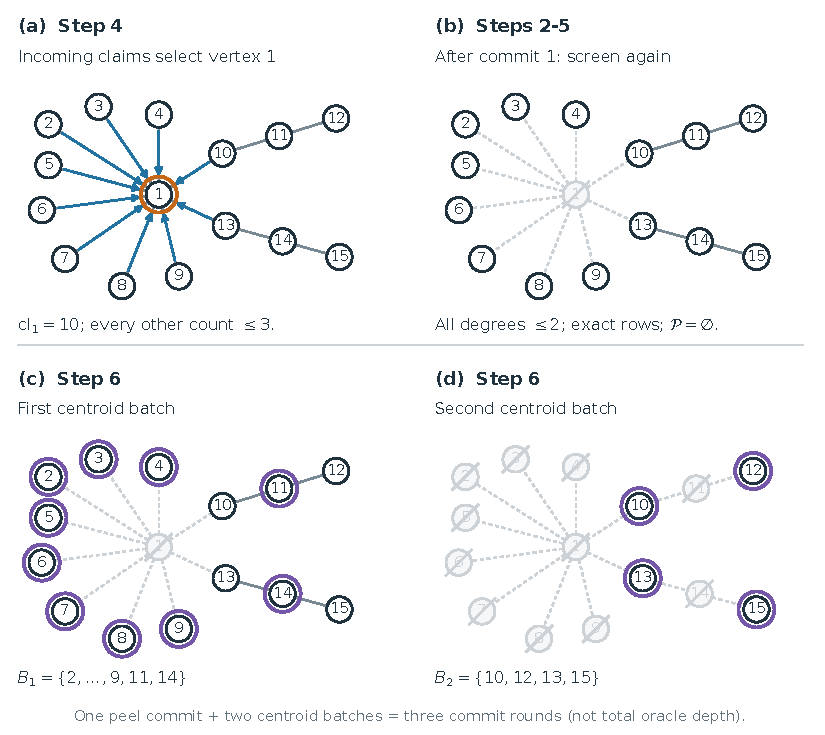
\includegraphics[width=\linewidth]{figures/algorithm_examples_2026-09-18/output/pdf/workflow_2026-09-18.pdf}
 \caption{The successful-screen path of
 \cref{ex:algorithm-peel-centroids-20260918}, with $N=15$ and $d=9$.
 Orange and violet rings denote the next peel or centroid commit;
 pale crossed vertices are already committed. The fills here are
 neutral, not random colors. The step labels refer to
 Algorithm~\ref{app:alg:complete-sampler}. A fresh screen separates (a) from (b);
 the terminal forest then needs no further discovery. All vertices
 remain individually visible.}
 \label{fig:algorithm-workflow-20260918}
\end{figure}


\paragraph{Intuition.}
A high-degree vertex that receives at most $\DegreeCutoff/2$ claims has
at most $\DegreeCutoff/2$ low-degree neighbors, because those neighbors
report it exactly.  It must therefore have more than $\DegreeCutoff/2$
neighbors inside the high-degree subforest.  A forest has fewer than
twice as many total degrees as vertices, so only a fraction at most
$4/\DegreeCutoff$ of high-degree vertices can survive one phase.
When $\DegreeCutoff=N^{\DegreeExponent+o(1)}$ with fixed
$\DegreeExponent>0$, the required number of phases is
$O_{\DegreeExponent}(1)$.

% Please keep this short statement together so its two stopping tests are visible.
\Needspace{12\baselineskip}
\begin{lemma}[Successful-path contraction and sound stopping\textcolor{red}{; \AlgoBlockRef{peel}, \AlgoBlockRef{terminal}}]
\label{app:lem:successful-path-structure}
Under the setup of Appendix~\ref{app:setup}, suppose preprocessing is feasible
and $\ScreenResolution<\EdgeSignal$.  Consider an execution path on which
every reached screen is successful in the sense of
\eqref{app:eq:screen-success-event}.  Let
$\HighDegreeCount{k}$ be the number of vertices whose residual degree exceeds
$\DegreeCutoff$ at the beginning of peel phase $k$.  After a nonempty peel
phase,
\begin{equation}
 \HighDegreeCount{k+1}
 \le\frac{4}{\DegreeCutoff}\HighDegreeCount{k},
 \label{app:eq:proof-peeling-contraction}
\end{equation}
with strict inequality whenever $\HighDegreeCount{k}>0$.
Moreover, either peel-loop stopping test in \AlgoBlockRef{peel} of
Algorithm~\ref{app:alg:complete-sampler}---an empty peel set or the
peel-phase cap---implies that the terminal residual
maximum degree is at most $\DegreeCutoff$.  The terminal certified graph is
therefore the true residual forest, so no cycle repair is performed.
\end{lemma}

\begin{proof}
\emph{1. High-degree neighbors of an unpeeled vertex.}
Fix a phase and define its high-degree set by
\begin{equation}
 \HighDegreeSet:=\{v\in\ResidualPositions:
                   d_{\ResidualForest}(v)>\DegreeCutoff\}.
 \label{app:eq:current-high-degree-set}
\end{equation}
At the beginning of phase $k$, $\HighDegreeCount{k}=|\HighDegreeSet|$.
Recall from \AlgoBlockNamedRef{peel} that the incoming claim count is
$\ClaimCount{v}=\sum_{u\in\ResidualPositions}\mathbf 1\{v\in\ScreenRow{u}\}$
and the peel threshold is $\ClaimCount{v}>\DegreeCutoff/2$.
For $v\in\HighDegreeSet\setminus\PeelSet$, every low-degree neighbor
reports $v$ exactly by \AppLowDegreeScreenRef.  Hence
\begin{align*}
 |\mathcal N_{\ResidualForest}(v)\setminus\HighDegreeSet|
 &=\sum_{u\in\ResidualPositions\setminus\HighDegreeSet}
       \mathbf 1\{v\in\mathcal N_{\ResidualForest}(u)\}\\
 &=\sum_{u\in\ResidualPositions\setminus\HighDegreeSet}
       \mathbf 1\{v\in\ScreenRow{u}\}
 \le\ClaimCount{v}\le\DegreeCutoff/2,\\
 d_{\ResidualForest[\HighDegreeSet]}(v)
 &=d_{\ResidualForest}(v)
       -|\mathcal N_{\ResidualForest}(v)\setminus\HighDegreeSet|\\
 &\ge d_{\ResidualForest}(v)-\ClaimCount{v}
 >\DegreeCutoff/2.
\end{align*}
The first equality uses the undirected nature of the forest.  Claims from
high-degree rows can only increase the incoming count, so they cannot
invalidate the bound for an unpeeled vertex.  We have shown that
\begin{equation}
 d_{\ResidualForest[\HighDegreeSet]}(v)
 >\frac{\DegreeCutoff}{2}.
 \label{app:eq:survivor-high-neighbors}
\end{equation}

\emph{2. Contraction after one peel phase.}
\emph{Empty survivor set.}
If $\HighDegreeSet\setminus\PeelSet=\emptyset$, no current high-degree vertex
survives the phase.  Deleting vertices cannot increase residual degrees, so
$\HighDegreeCount{k+1}=0$; this proves
\eqref{app:eq:proof-peeling-contraction}, strictly when
$\HighDegreeSet\ne\emptyset$.

\emph{Nonempty survivor set.}
Suppose instead that $\HighDegreeSet\setminus\PeelSet\ne\emptyset$.
Summing \eqref{app:eq:survivor-high-neighbors} over these unpeeled high-degree
vertices and using the forest degree-sum identity in
\cref{app:lem:forest-basics} gives
\begin{equation}
 \frac{\DegreeCutoff}{2}
 |\HighDegreeSet\setminus\PeelSet|
 <\sum_{v\in\HighDegreeSet\setminus\PeelSet}
   d_{\ResidualForest[\HighDegreeSet]}(v)
 \le2|E(\ResidualForest[\HighDegreeSet])|
 <2|\HighDegreeSet|.
 \label{app:eq:proof-high-degree-sum}
\end{equation}
Let $H'=(G',x_{G'})$ be the history after all singleton commits in the frozen
peel set of this phase, and recall the induced residual forest
$\ResidualForestAt{G'}=\TargetForest[\ResidualPositionsAt{G'}]$ from
\eqref{app:eq:history}.  Define
$\HighDegreeSetAt{H'}:=\{v\in\ResidualPositionsAt{G'}:
 d_{\ResidualForestAt{G'}}(v)>\DegreeCutoff\}$.
Deleting vertices cannot increase residual degrees:
\[
 \HighDegreeSetAt{H'}\subseteq\HighDegreeSet\setminus\PeelSet,
 \qquad
 \HighDegreeCount{k+1}=|\HighDegreeSetAt{H'}|
 \le|\HighDegreeSet\setminus\PeelSet|.
\]
Dividing \eqref{app:eq:proof-high-degree-sum} by $\DegreeCutoff/2$ now gives
$|\HighDegreeSet\setminus\PeelSet|<(4/\DegreeCutoff)|\HighDegreeSet|$,
and hence the strict form of \eqref{app:eq:proof-peeling-contraction}.  If
$\HighDegreeSet=\emptyset$, then the first case above gives equality
$\HighDegreeCount{k+1}=\HighDegreeCount{k}=0$.

\emph{3. Sound stopping at the phase cap.}
Initially, \cref{app:lem:forest-basics} makes the forest degree sum smaller
than $2N$, while each high-degree vertex has degree at least
$\DegreeCutoff+1$.  Hence
\begin{equation}
 \HighDegreeCount{0}<\frac{2N}{\DegreeCutoff+1}.
 \label{app:eq:initial-high-count}
\end{equation}
If the right-hand side is at most one, integrality already gives
$\HighDegreeCount{0}=0$.
Otherwise, once $\HighDegreeCount{k}=0$, deleting further vertices keeps every
later high-degree count equal to zero.  If this never occurs before the phase
cap, then $\HighDegreeCount{k}>0$ in every preceding phase, so the strict part
of \eqref{app:eq:proof-peeling-contraction} may be iterated.  In either case,
after $\PeelPhaseCap$ completed phases,
\begin{equation}
 \HighDegreeCount{\PeelPhaseCap}
 <\left(\frac4{\DegreeCutoff}\right)^{\PeelPhaseCap}
   \frac{2N}{\DegreeCutoff+1}
 \le
 \left(\frac8{\DegreeCutoff}\right)^{\PeelPhaseCap}
   \frac{2N}{\DegreeCutoff+1}
 \le1,
 \label{app:eq:phase-cap-eliminates-high-core}
\end{equation}
To check the last inequality, $\DegreeCutoff\ge9$ gives
$\log(\DegreeCutoff/8)>0$, and the ceiling in
\eqref{app:eq:phase-cap} gives
\begin{align*}
 \PeelPhaseCap\log(\DegreeCutoff/8)
 &\ge \PositivePart{\log(2N/(\DegreeCutoff+1))},\\
 \left(\frac8{\DegreeCutoff}\right)^{\PeelPhaseCap}
       \frac{2N}{\DegreeCutoff+1}
 &=\exp\!\left\{\log\frac{2N}{\DegreeCutoff+1}
                -\PeelPhaseCap\log(\DegreeCutoff/8)\right\}\le1.
\end{align*}
The integer in \eqref{app:eq:phase-cap-eliminates-high-core} is therefore zero.

\emph{4. Sound stopping with an empty peel set.}
If instead $\PeelSet=\emptyset$ while $\HighDegreeSet$ is nonempty, then
\eqref{app:eq:proof-high-degree-sum} holds with
$\HighDegreeSet\setminus\PeelSet=\HighDegreeSet$.  It would imply
$\DegreeCutoff/2<2$, contradicting $\DegreeCutoff\ge9$.  Hence an empty peel
set also certifies the absence of high-degree vertices.

\emph{5. \textcolor{red}{Bound peel-set size and certify the terminal graph.}}
We first check that the hard round cap cannot interrupt peeling.
\textcolor{red}{Fix a phase at history $\History$ with
$n:=|\ResidualPositions|\ge1$; if no vertex remains, the algorithm has
already returned.}
Low-degree exactness\textcolor{red}{~(\AppLowDegreeScreenRef)} and the row-size cap\textcolor{red}{~%
(\cref{app:def:row-selector})} imply
$|\ScreenRow{u}|\le d_{\ResidualForest}(u)$ for every $u$:
there is equality at low degree, while
$|\ScreenRow{u}|\le\DegreeCutoff<d_{\ResidualForest}(u)$ at high degree.
Counting each reported ordered pair once\textcolor{red}{, first at its
recipient and then in its reporting row,} gives
{\color{red}
\begin{align}
 \sum_{v\in\ResidualPositions}\ClaimCount{v}
 &=\sum_{v\in\ResidualPositions}\sum_{u\in\ResidualPositions}
       \mathbf 1\{v\in\ScreenRow{u}\}\notag\\
 &=\sum_{u\in\ResidualPositions}\sum_{v\in\ResidualPositions}
       \mathbf 1\{v\in\ScreenRow{u}\}\notag\\
 &=\sum_{u\in\ResidualPositions}|\ScreenRow{u}|\notag\\
 &\le\sum_{u\in\ResidualPositions}d_{\ResidualForest}(u)
 =2|E(\ResidualForest)|<2n.
 \label{app:eq:total-claim-bound}
\end{align}}
\textcolor{red}{The second equality interchanges finite sums; the last line
uses the forest degree sum in \cref{app:lem:forest-basics}.
Recall $\PeelSet=\{v\in\ResidualPositions:\ClaimCount{v}>\DegreeCutoff/2\}$
from \cref{app:eq:claim-and-peel-set}.
If $\PeelSet=\emptyset$, then $|\PeelSet|=0<4n/\DegreeCutoff$.
Otherwise its strict threshold gives}
{\color{red}
\begin{equation}
 \begin{aligned}
 \frac{\DegreeCutoff}{2}|\PeelSet|
 &<\sum_{v\in\PeelSet}\ClaimCount{v}
 \le\sum_{v\in\ResidualPositions}\ClaimCount{v}<2n,\\
 |\PeelSet|&<\frac{4n}{\DegreeCutoff}\le\frac{4N}{\DegreeCutoff}.
 \end{aligned}
 \label{app:eq:peel-set-size-proof}
\end{equation}}
\textcolor{red}{\AlgoBlockNamedRef{peel} freezes this set before its singleton
commits, so the phase uses exactly $|\PeelSet|$ rounds if completed and no
more if interrupted.}
With at most $\PeelPhaseCap$ phases, immediately before any planned peel
commit the completed-round counter satisfies
{\color{red}
\begin{equation}
 r<\frac{4N\PeelPhaseCap}{\DegreeCutoff}<\HardRoundCap-1,
 \label{app:eq:peel-before-hard-cap}
\end{equation}}
by \eqref{app:eq:screen-call-and-round-caps}.
\textcolor{red}{Thus \AlgoGuardRef\ cannot interrupt peeling.}
If all positions have already been committed, the residual graph is empty.
Otherwise peeling reaches one of the two tests identified in the statement.
Each pass executes \AlgoBlockRef{screen} before either stopping test
in \AlgoBlockRef{peel}.  At the
terminal history every residual vertex is consequently covered by
\AppLowDegreeScreenRef; the terminal screen is successful by
hypothesis, so all terminal rows are exact.  The
symmetrized edge set in \AlgoBlockNamedRef{terminal} is therefore
exactly $E(\ResidualForestAt{\star})$.  In particular, the cycle-repair loop
is skipped on the successful path.
\end{proof}

\begin{example}[A high-degree vertex can survive a peel phase]
\label{ex:algorithm-survivor-20260918}
This separate example illustrates the row contract used in
\cref{app:lem:successful-path-structure}, rather than specifying a
target--oracle pair.  Let $\DegreeCutoff=9$ and take the $65$ vertices
\[
 U=\{z\}\cup\{h_i:1\le i\le6\}
   \cup\{u_{i,j}:1\le i\le6,\ 1\le j\le9\}
   \cup\{s_1,s_2,s_3,s_4\},
\]
with edges
\[
 E=\{\{z,h_i\}:1\le i\le6\}
 \cup\{\{h_i,u_{i,j}\}:1\le i\le6,\ 1\le j\le9\}
 \cup\{\{z,s_j\}:1\le j\le4\}.
\]
At the history under consideration, take $\ResidualPositions=U$ and
$\ResidualForest=F=(U,E)$.
The center $z$ and all six hubs have degree $10$; all other vertices
are leaves.  Take the following row outputs, which obey the contract
\emph{exact at degree at most $d$, size at most $d$ elsewhere}:
\[
 \ScreenRow{z}=\ScreenRow{h_i}=\emptyset,\qquad
 \ScreenRow{u_{i,j}}=\{h_i\},\qquad
 \ScreenRow{s_j}=\{z\}.
\]
Computing the incoming counts, rather than reading a high-degree row's
size as its degree, gives
\begin{align*}
 \ClaimCount{z}&=4\le9/2, & \ClaimCount{h_i}&=9>9/2,\\
 \ClaimCount{u_{i,j}}&=\ClaimCount{s_j}=0,
 & \PeelSet&=\{h_1,\ldots,h_6\}.
\end{align*}
Thus $z$ is not peeled.  Before the commits its high-degree neighbors
are exactly $\{h_1,\ldots,h_6\}$, so their number is $6>9/2$, as required by
\eqref{app:eq:survivor-high-neighbors}.  After the six frozen singleton
commits in \AlgoBlockRef{peel}, its remaining neighbors are $\{s_1,\ldots,s_4\}$:
\begin{align*}
 d_{F[U\setminus\PeelSet]}(z)&=4,\\
 |\{v\in U:d_F(v)>9\}|&=7,\\
 |\{v\in U\setminus\PeelSet:d_{F[U\setminus\PeelSet]}(v)>9\}|&=0.
\end{align*}
The center survives as a vertex but ceases to be high-degree.
The $54$ hub leaves become isolated; none was committed in this phase.
\Cref{fig:algorithm-survivor-20260918} draws each of them separately.
\end{example}

\begin{figure}[H]
 \centering
 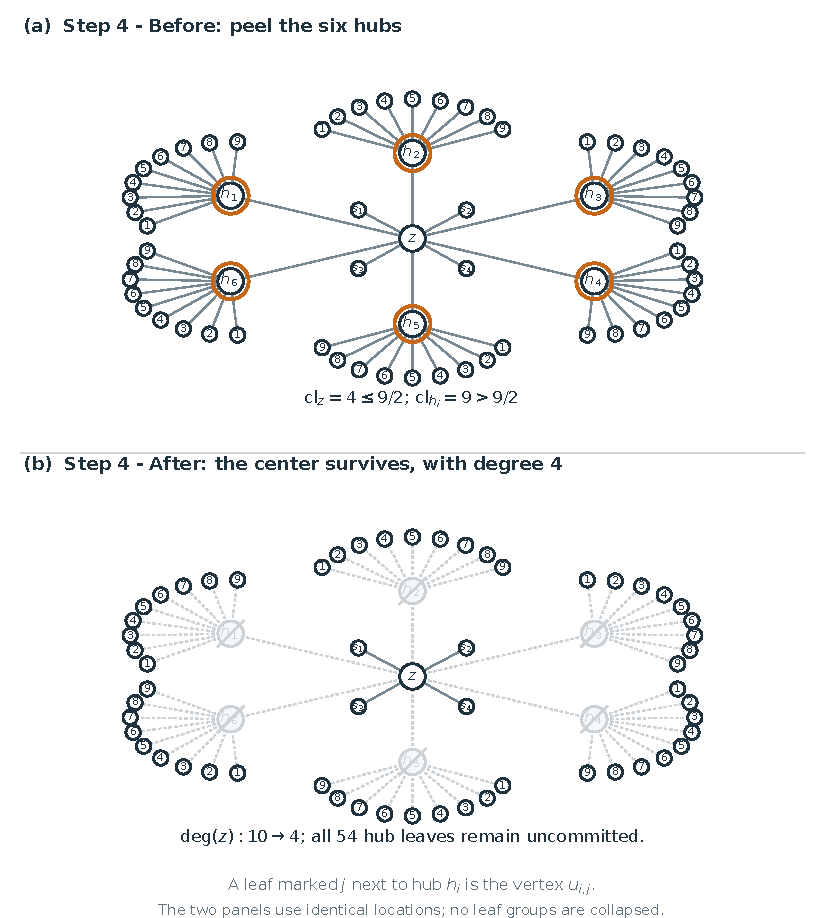
\includegraphics[width=\linewidth]{figures/algorithm_examples_2026-09-18/output/pdf/survivor_2026-09-18.pdf}
 \caption{The separate contraction example of
 \cref{ex:algorithm-survivor-20260918}. The six orange-ringed hubs are
 committed one at a time in \AlgoBlockRef{peel}, with no intervening screen or peel-set
 recomputation. Their $54$ leaves are drawn individually, not bundled.
 The unpeeled center $z$ changes from degree $10$ to degree $4$.
 The lower panel keeps the same locations and crosses out only the
 committed hubs.}
 \label{fig:algorithm-survivor-20260918}
\end{figure}


\paragraph{Intuition.}
\textcolor{red}{The total counterfactual-submission count is bounded by the
product of the screen-loop bounds:}
\[
 \textcolor{red}{\CounterfactualQueries\le}
 \underbrace{\ScreenColumnCount}_{\text{\textcolor{red}{source columns}}}\qquad
 \underbrace{\ScreenCallCap}_{\text{\textcolor{red}{screen calls}}}\qquad
 \underbrace{\RandomColoringCount}_{\text{\textcolor{red}{colorings/screen}}}\qquad
 \underbrace{\RandomColorCount}_{\text{source colors}}\qquad
 \underbrace{(\RandomColorCount+\ChunkCount)}_{\text{\textcolor{red}{chunks/coloring}}}.
\]
For rounds, \textcolor{red}{\cref{app:eq:peel-set-size-proof} bounds each peel set by}
$4N/\DegreeCutoff$; after the peel phases, centroid recursion needs only
$\lceil\log_2(N+1)\rceil$ layers.  The public cap extends the round bound to
failed-screen paths.  Total masked-state submissions, including
preprocessing and commits, are $\CounterfactualQueries+\CommitRounds+1$.

% Please keep the resource statement from starting with only two lines at a page foot.
\Needspace{14\baselineskip}
\begin{lemma}[Finite query and round counts\textcolor{red}{; \AlgoBlockRef{preprocess}--\AlgoBlockRef{centroid}}]
\label{app:lem:upper-resources}
Suppose preprocessing is feasible and
$\ScreenResolution<\EdgeSignal$.  On every execution path of
$\SelectedPackedSampler$ with any admissible row selector and the standard draft generator,
\begin{align}
 \CounterfactualQueries
 &\le\ScreenColumnCount\ScreenCallCap\RandomColoringCount
       \RandomColorCount(\RandomColorCount+\ChunkCount),
 \label{app:eq:proof-finite-Q}\\
 \CommitRounds
 &\le\HardRoundCap.
 \label{app:eq:proof-finite-R}
\end{align}
where
$\HardRoundCap=\lceil4N\PeelPhaseCap/\DegreeCutoff\rceil
+\lceil\log_2(N+1)\rceil+2$ is the public commit-round cap and
$\ScreenCallCap=\PeelPhaseCap+1$ is the screen-call cap from
\eqref{app:eq:screen-call-and-round-caps};
$\PeelPhaseCap$ is the peel-phase cap in \eqref{app:eq:phase-cap}.
In \eqref{app:eq:proof-finite-Q}, $\RandomColorCount$ and
$\RandomColoringCount$ are the fixed numbers of colors and independent
colorings per screen from \eqref{app:eq:random-color-parameters}.
The subscript $\mathrm{rnd}$ labels the randomized-color construction,
not a round index.
On a path on which every reached screen is successful, the sharper bound
\begin{equation}
 \CommitRounds
 <\frac{4N\PeelPhaseCap}{\DegreeCutoff}
   +\left\lceil\log_2(N+1)\right\rceil
 \label{app:eq:successful-path-rounds}
\end{equation}
holds, with no cycle repair or round-cap fallback.
The adaptive oracle depth, including the initial all-mask preprocessing
stage, satisfies
\begin{equation}
 \OracleDepth\le1+\CommitRounds+\ScreenCallCap.
 \label{app:eq:finite-oracle-depth}
\end{equation}
\end{lemma}

\begin{proof}

\emph{1. Count submissions over chunks, columns, and screens.}
Fix one screen execution at history $\History$.  Recall the quantities
counted in its loops:
\begin{itemize}
\item $\ScreenQueries$ denotes the number of masked-state submissions in
this one call to \AlgoBlockNamedRef{screen}, all made in
\AlgoBlockRef{probes}; preprocessing and commit submissions are excluded.
\item $\MaxBankSize=\max_{i\in\PositionSet}|\TokenBank{i}|$ is the largest
local vocabulary-bank size fixed in \cref{app:def:preprocessing}.
The number of submitted source columns is
$\ScreenColumnCount=\MaxBankSize+1$ when $\MaxBankSize\ge1$, and
$\ScreenColumnCount=0$ otherwise, as in \eqref{app:eq:screen-column-count}.
\item $\ColorCount=\RandomColorCount=8(\DegreeCutoff+1)$ is the number of
colors, and $\ColoringCount=\RandomColoringCount$ is the number of
independent colorings supplied by \AlgoBlockNamedRef{draft};
their choices are \eqref{app:eq:random-color-parameters}.
\item $\ChunkCount\in\PositionSet$ is the readout-chunk parameter from
\cref{app:algorithm-overview}: it sets
$\ReadoutChunkSize=\lceil N/\ChunkCount\rceil$, the maximum chunk size.
It is not the actual number of chunks.
\end{itemize}
For one coloring $\tau$, write $n_c:=|\ColorClass{\tau}{c}|$ and let
$\ChunksPerColoring{\tau}$ be the total number of readout chunks across
its color classes.  The deterministic partition
\eqref{app:eq:readout-chunks} in \AlgoBlockRef{chunks} creates exactly
$\lceil n_c/\ReadoutChunkSize\rceil$ chunks for every nonempty color class.
Therefore
\begin{align}
 \ChunksPerColoring{\tau}
 &=\sum_{c:n_c>0}
   \left\lceil\frac{n_c}{\ReadoutChunkSize}\right\rceil\notag\\
 &\le\sum_{c:n_c>0}
   \left(1+\frac{n_c}{\ReadoutChunkSize}\right)\notag\\
 &\le\ColorCount+\frac{|\ResidualPositions|}{\ReadoutChunkSize}
 \le\ColorCount+\ChunkCount.
 \label{app:eq:proof-chunk-count}
\end{align}
For each chunk, the bank columns and source-specific tail column in
\AlgoBlockRef{probes} use
$(\MaxBankSize+1)(\ColorCount-1)$ submissions.  When
$\MaxBankSize\ge1$, this is at most
$\ScreenColumnCount\ColorCount$.  Thus \AlgoBlockRef{chunks} supplies at
most $\ColorCount+\ChunkCount$ chunks per coloring, and
\AlgoBlockRef{probes} submits at most $\ScreenColumnCount\ColorCount$
states per chunk.  Summing over the $\ColoringCount$ colorings from
\AlgoBlockRef{draft} gives
\begin{equation}
 \ScreenQueries
 \le
 \underbrace{\ScreenColumnCount}_{\text{\textcolor{red}{source columns}}}\qquad
 \underbrace{\ColoringCount}_{\text{\textcolor{red}{colorings/screen}}}\qquad
 \underbrace{\ColorCount}_{\text{source colors}}\qquad
 \underbrace{(\ColorCount+\ChunkCount)}_{\text{chunks per coloring}}.
 \label{app:eq:proof-one-screen-count}
\end{equation}
When $\MaxBankSize=0$, the algorithm submits no screen state and both sides
are zero.  The screen runs initially and once after each of at most
$\PeelPhaseCap$ completed peel phases, hence at most $\ScreenCallCap$ times.
Substituting the randomized values of $\ColoringCount$ and $\ColorCount$
proves \eqref{app:eq:proof-finite-Q}.  The standard draft reuses preprocessing
and adds no query. Cycle repair runs no further screen: each singleton
repair is one commit submission, charged to $\CommitRounds$, not to
$\CounterfactualQueries$.

\emph{Returned oracle rows.}
For the standard zero-query draft, each counterfactual submission reads
only its chunk, of size at most $\ReadoutChunkSize=\lceil N/\ChunkCount\rceil$.
Preprocessing reads $N$ rows, and the disjoint commit batches
$B_1,\ldots,B_{\CommitRounds}$ partition $\PositionSet$
(\cref{app:def:admissible-algorithm}), so $\sum_{t=1}^{\CommitRounds}|B_t|=N$.
The main construction takes $\ChunkCount=\DegreeCutoff$.
Consequently the total number of returned oracle rows is at most
\[
 \underbrace{\lceil N/\ChunkCount\rceil\CounterfactualQueries}_{\text{screen submissions}}
 +\underbrace{N}_{\text{preprocessing}}
 +\underbrace{\sum_{t=1}^{\CommitRounds}|B_t|}_{\text{commits}}
 =\lceil N/\ChunkCount\rceil\CounterfactualQueries+2N.
\]


\emph{2. Count adaptive oracle stages.}
Once the history, draft, and colors are fixed, all submissions in a screen
can be issued in one parallel oracle stage \textcolor{red}{in
\AlgoBlockRef{probes}, because their states do not depend on replies from
that screen}.  Each commit requires one stage,
and preprocessing \textcolor{red}{in \AlgoBlockRef{preprocess}} requires one. This proves
\eqref{app:eq:finite-oracle-depth}.


\emph{3. Bound peeling rounds on a successful path.}
\textcolor{red}{On a path where every reached screen succeeds,
\eqref{app:eq:peel-set-size-proof} in
\cref{app:lem:successful-path-structure} shows that every nonempty peel phase in
\AlgoBlockNamedRef{peel} commits fewer than $4N/\DegreeCutoff$ vertices,
one per round.  At most $\PeelPhaseCap$ such phases therefore use fewer than
$4N\PeelPhaseCap/\DegreeCutoff$ rounds.
The bound \eqref{app:eq:peel-before-hard-cap} also shows that
\AlgoGuardRef\ cannot interrupt these commits.}


\emph{4. Bound terminal centroid rounds and exclude repair and fallback.}
By Lemma~\ref{app:lem:successful-path-structure}, the terminal certified graph
is the true residual forest.  Lemma~\ref{app:lem:residual-markov} makes its
connected components conditionally independent.  At any layer of
\AlgoBlockNamedRef{centroid}, let
the current components be $T_1,\ldots,T_m$, with selected centroids
$\ComponentCentroid{1},\ldots,\ComponentCentroid{m}$, and set
$B=\{\ComponentCentroid{1},\ldots,\ComponentCentroid{m}\}$.  Then
\begin{equation}
 \TargetLaw(X_B=x_B\mid X_G=x_G)
 =\prod_{\ell=1}^m
   \TargetLaw\bigl(X_{\ComponentCentroid{\ell}}
   =x_{\ComponentCentroid{\ell}}\mid X_G=x_G\bigr).
 \label{app:eq:centroid-batch-factorization}
\end{equation}
Thus their exact singleton rows define the exact joint batch conditional.
By
\cref{app:lem:forest-basics}, removing a centroid leaves components of size at
most half the parent size, so after
$\ell$ terminal batches every remaining component has size at most $N/2^\ell$.
For $\ell=\lceil\log_2(N+1)\rceil$ this is smaller than one.  Adding the peeling
and terminal rounds proves \eqref{app:eq:successful-path-rounds}.  Its
right-hand side is smaller than $\HardRoundCap-1$ by
\eqref{app:eq:screen-call-and-round-caps}; hence the hard-cap check is never
triggered during the terminal stage either. The terminal graph is already
a forest, so the cycle-repair loop adds no rounds.


\emph{5. Enforce the round cap on every path.}
It remains to verify the unconditional randomized round bound enforced by
\AlgoGuardRef. Initially $r=0\le\HardRoundCap-1$. Before every peel, repair,
or centroid commit, the algorithm checks whether $r=\HardRoundCap-1$.
If equality holds, it commits all remaining positions in the reserved
final round and returns. Otherwise the integer counter satisfies
$r\le\HardRoundCap-2$, and the next commit leaves
$r+1\le\HardRoundCap-1$.
Every such commit is nonempty and irrevocable, so it removes at least
one remaining position; cycle repair cannot continue indefinitely.
If it ends without the cap fallback, the remaining working graph is a
forest and centroid completion applies. Induction over commit operations
therefore gives $\CommitRounds\le\HardRoundCap$ on every path, proving
\eqref{app:eq:proof-finite-R}.
\end{proof}

\subsection{Exact-commit hybrid and adaptive error composition}
\label{app:upper-proof-error}

This subsection completes the statistical part of the upper bound.
\Cref{app:lem:exact-hybrid} identifies a structurally safe exact-row hybrid
with the target law.  Separately,
\cref{app:lem:adaptive-hellinger-upper} bounds the distance between any
product-commit decision rule and its exact-row hybrid, whether or not its
batches are structurally safe.  A safe-decision-rule comparison then accounts
for failed screens in the implemented randomized sampler.


\paragraph{Structural safety.}
At a history $\History=(G,x_G)$, let $\ResidualForest$ be the true residual
forest on $\ResidualPositions=\PositionSet\setminus G$.
A complete decision rule is \emph{structurally safe} if, at every realized
history, each batch $B\subseteq\ResidualPositions$ it commits satisfies
\[
 |B\cap V(T)|\le1
 \qquad\text{for every connected component }T\text{ of }\ResidualForest.
\]
In particular, every singleton batch is safe.
This is a property used in the analysis, not permission for the implemented
sampler to inspect the hidden forest.

\paragraph{The two executions and their output laws.}
Fix one complete decision rule, the frozen oracle $\FrozenOracle$, and a
decision-rule seed $\ControllerSeed=w$, including the colors and all
auxiliary draft randomness.  The product-commit draws remain random after
this conditioning.  For a chosen batch $B$ and the history-compatible
commit state $y$ in \eqref{app:eq:commit-state}, compare:
\begin{itemize}
\item \emph{Oracle execution.}
A batch assignment $z\in\Vocab^B$ has mass
$\prod_{j\in B}\OracleRowMass{y}{j}{z_j}$.
Recall from \textcolor{red}{\cref{app:def:output-risk}} that its full output law is
$\SamplerOutputLaw{w}{\FrozenOracle}(x)
 =\Pr(\SamplerOutput=x\mid\ControllerSeed=w)$, with $\FrozenOracle$ fixed
and all product-commit draws integrated out.
\item \emph{Exact-commit hybrid.}
Replace only this commit mass by
$\prod_{j\in B}\ExactRowMass{y}{j}{z_j}$, using the exact rows in
\eqref{app:eq:exact-row}.  Keep the decision rule, draft generator, query
rules, and all frozen-oracle replies unchanged.
Denote this execution's full output law by $\ExactCommitOutputLaw{w}$.
\end{itemize}
Both are laws on $\Vocab^N$; $\otimes$ refers to the product within each
commit, not to independence of all output coordinates.
The hybrid can still depend on $\FrozenOracle$ through its decisions;
that dependence is suppressed in $\ExactCommitOutputLaw{w}$.
The shared rules do not imply shared realized transcripts: different commit
outcomes can lead to different later queries and batches.

Structural safety identifies the hybrid's product at each commit with the
target's joint batch conditional; for an unsafe batch they need not agree.
Thus \cref{app:lem:exact-hybrid} uses safety to prove
$\ExactCommitOutputLaw{w}=\TargetLaw$, whereas
\cref{app:lem:adaptive-hellinger-upper} compares the two output laws without
requiring safety.  Both lemmas also apply to the analysis-only decision rule
introduced below.

\paragraph{Intuition.}
A safe batch takes at most one vertex from each independent residual
component.  Its product of exact rows is therefore the exact joint
conditional.  Multiplying these joint conditionals along the adaptive
partition is the ordinary chain rule, so the output law is exactly
$\TargetLaw$.

\begin{lemma}[Exact hybrid equals the target law]
\label{app:lem:exact-hybrid}
For every structurally safe complete decision rule, the exact-commit hybrid
satisfies
\begin{equation}
 \ExactCommitOutputLaw{w}=\TargetLaw
 \qquad\text{for every decision-rule seed }w.
 \label{app:eq:exact-hybrid-target}
\end{equation}
\end{lemma}

\begin{proof}

\emph{1. Identify the exact joint law of a safe batch.}
For a singleton batch the product of exact singleton rows is trivially its
exact joint conditional.  For a nonsingleton safe batch, its vertices lie in
distinct true residual components.  Lemma~\ref{app:lem:residual-markov}
therefore identifies their exact joint conditional with the product of their
exact singleton conditionals, as in
\eqref{app:eq:centroid-batch-factorization}.


\emph{2. Apply the chain rule along each adaptive path.}
For fixed $w$, draft generation is deterministic as a function of the observed
past, even when its rule is randomized before conditioning on $w$.
For a full assignment $x\in\Vocab^N$, let $B_t(x)$ be the batch selected along
the unique hybrid path consistent with $x$, and let $G_{t-1}(x)$ be the set
committed before that batch, with $G_0(x)=\varnothing$ and
$G_t(x)=G_{t-1}(x)\cup B_t(x)$.  The batches form an adaptive ordered partition
of $\PositionSet$.  The preceding paragraph identifies every hybrid batch law
with the corresponding exact joint conditional, so the conditional chain
rule gives
\begin{align}
 \ExactCommitOutputLaw{w}(x)
 &=\prod_t
 \TargetLaw\!\left(
  X_{B_t(x)}=x_{B_t(x)}
 \mid X_{G_{t-1}(x)}=x_{G_{t-1}(x)}
 \right)\notag\\
 &=\prod_t
 \frac{\TargetLaw(X_{G_t(x)}=x_{G_t(x)})}
      {\TargetLaw(X_{G_{t-1}(x)}=x_{G_{t-1}(x)})}\notag\\
 &=\TargetLaw(x).
 \label{app:eq:adaptive-exact-chain-rule}
\end{align}
The batch partition may depend on earlier committed values, but for each fixed
$x$ the displayed factors are precisely the chain-rule factors along that
path.  Consecutive numerators and denominators cancel; the first denominator
is the probability of the empty constraint, hence one, and the last numerator
is $\TargetLaw(x)$ because every coordinate has been committed.
This proves the equality pointwise.
\end{proof}

We next compare the full output laws $\ExactCommitOutputLaw{w}$ (exact-row
commits) and $\SamplerOutputLaw{w}{\FrozenOracle}$ (oracle-row commits) for
the same decision rule and fixed seed.  For probability masses $P,Q$ on a
finite set, write
\begin{equation}
 \HellingerAffinity(P,Q)
 :=\sum_x\sqrt{P(x)Q(x)}
 =1-\sqHellinger(P,Q).
 \label{app:eq:affinity-definition}
\end{equation}

\paragraph{Intuition.}
The error budget is attached to committed coordinates, not to probes or
rounds.  Each coordinate is committed once, so the total budget is
\[
 N\cdot\frac{(\OracleRadius)^2}{2N}=\frac{(\OracleRadius)^2}{2}.
\]
For adaptive batches, backward induction on the execution tree justifies
this accounting.  At each node, charge the current batch and then use the
budget of the remaining coordinates.

\begin{lemma}[Adaptive squared-Hellinger composition]
\label{app:lem:adaptive-hellinger-upper}
{\color{red}Assume \cref{app:ass:oracle-accuracy} (A2): every valid row pair obeys
$\sqHellinger(\ExactRow{y}{j},\OracleRow{y}{j})
 \le(\OracleRadius)^2/(2N)$.  For every complete decision rule using the
product-commit rule and every fixed decision-rule seed $w$, regardless of
structural safety,}
\begin{equation}
 \sqHellinger\bigl(
  \ExactCommitOutputLaw{w},
  \SamplerOutputLaw{w}{\FrozenOracle}
 \bigr)
 \le\frac{(\OracleRadius)^2}{2}.
 \label{app:eq:global-upper-hellinger}
\end{equation}
\end{lemma}

\begin{proof}

\emph{1. Compare the two kernels at a common node.}
Fix $\FrozenOracle$ and $w$ throughout the proof.
\hypertarget{app-execution-tree-state}{}
An \emph{execution-tree node} is a stored algorithm state immediately before
a commit, or a terminal state after completion; it is not a vertex of the
hidden forest.  A pre-commit state records
\[
 \mathfrak h=(\History,\ScreenTranscript,\text{decision-rule state}),
 \qquad
 \History=(G,x_G),\quad
 \ResidualPositions=\PositionSet\setminus G.
\]
Here $\ScreenTranscript$ contains the preceding query/reply and commit
record, and the internal state includes any current draft and counters.
We use this complete stored state to define continuation kernels directly,
without replaying the decision rule from its initial state.
With $\FrozenOracle$ and $w$ fixed, all operations between commits are
deterministic.  Thus, from the \emph{same stored state} $\mathfrak h$, both
executions receive the same frozen-oracle replies and select the same
batch $B(\mathfrak h)\subseteq\ResidualPositions$ and commit state
$y(\mathfrak h)$ from \eqref{app:eq:commit-state}.
Comparing kernels at this common state does not assert that two separately
sampled executions have identical paths.
For a batch assignment $z\in\Vocab^{B(\mathfrak h)}$, their kernels are
\begin{align}
 \ExactBatchMass{\mathfrak h}{z}
 &:=\prod_{j\in B(\mathfrak h)}
       \ExactRowMass{y(\mathfrak h)}{j}{z_j},\notag\\
 \OracleBatchMass{\mathfrak h}{z}
 &:=\prod_{j\in B(\mathfrak h)}
       \OracleRowMass{y(\mathfrak h)}{j}{z_j}.
 \label{app:eq:exact-oracle-batch-laws}
\end{align}
Both kernels are probability masses on $\Vocab^{B(\mathfrak h)}$:
\begin{align*}
 \sum_{z\in\Vocab^{B(\mathfrak h)}}\ExactBatchMass{\mathfrak h}{z}
 &=\prod_{j\in B(\mathfrak h)}
       \sum_{a\in\Vocab}\ExactRowMass{y(\mathfrak h)}{j}{a}=1,\\
 \sum_{z\in\Vocab^{B(\mathfrak h)}}\OracleBatchMass{\mathfrak h}{z}
 &=\prod_{j\in B(\mathfrak h)}
       \sum_{a\in\Vocab}\OracleRowMass{y(\mathfrak h)}{j}{a}=1.
\end{align*}
The finite sums factor by distributivity over the Cartesian product.
The first kernel is a product of exact rows, whether or not it equals the
target's joint batch conditional.  \textcolor{red}{Hence this comparison needs
no structural safety condition.}


\emph{2. Charge the current batch to its coordinates.}
Apply the product identity in \cref{app:lem:finite-hellinger-calculus}
with index set $B(\mathfrak h)$, each coordinate space equal to $\Vocab$,
and component laws $\ExactRow{y(\mathfrak h)}{j}$ and
$\OracleRow{y(\mathfrak h)}{j}$.  This gives
\begin{equation}
 \HellingerAffinity(\ExactBatchLaw{\mathfrak h},
                    \OracleBatchLaw{\mathfrak h})
 =\prod_{j\in B(\mathfrak h)}
  \left[1-\sqHellinger\bigl(
        \ExactRow{y(\mathfrak h)}{j},
        \OracleRow{y(\mathfrak h)}{j}\bigr)\right].
 \label{app:eq:upper-batch-affinity}
\end{equation}
Using $1-\prod_j(1-u_j)\le\sum_j u_j$ for $u_j\in[0,1]$ and
\textcolor{red}{\eqref{app:eq:A2}},
\begin{align}
 1-\HellingerAffinity(\ExactBatchLaw{\mathfrak h},
                      \OracleBatchLaw{\mathfrak h})
 &=\sqHellinger(\ExactBatchLaw{\mathfrak h},
                \OracleBatchLaw{\mathfrak h})
 \label{app:eq:local-batch-cost-definition}\\
 &\le\sum_{j\in B(\mathfrak h)}
     \sqHellinger\bigl(\ExactRow{y(\mathfrak h)}{j},
                      \OracleRow{y(\mathfrak h)}{j}\bigr)\notag\\
 &\le |B(\mathfrak h)|\frac{(\OracleRadius)^2}{2N}.
 \label{app:eq:local-batch-cost-bound}
\end{align}


\emph{3. Derive the suffix-affinity recursion.}
Take a stored execution state $\mathfrak h$ from part~1 of this proof, with committed
history $\History=(G,x_G)$ and remaining set
$\ResidualPositions=\PositionSet\setminus G$.
Here a \emph{suffix} is the assignment of all still-uncommitted coordinates,
not necessarily a contiguous block of positions.  Define:
\begin{itemize}
\item $\ExactSuffixLaw{\mathfrak h}$: the law of those remaining values
when execution resumes from this entire stored state using exact-row commits.
\item $\OracleSuffixLaw{\mathfrak h}$: the corresponding law when it
resumes from the same state using oracle-row commits.
\end{itemize}
Both are probability laws on $\Vocab^{\ResidualPositions}$, with
$\FrozenOracle$ and $w$ still fixed.  The recursion below defines these
continuation laws from the batch kernels in
\eqref{app:eq:exact-oracle-batch-laws}; at a terminal state
$\ResidualPositions=\varnothing$, each puts mass one on the empty assignment.
Set
\begin{equation}
 \SuffixAffinity{\mathfrak h}
 :=\HellingerAffinity(\ExactSuffixLaw{\mathfrak h},
                      \OracleSuffixLaw{\mathfrak h}).
 \label{app:eq:suffix-affinity}
\end{equation}
After a batch value $z\in\Vocab^{B(\mathfrak h)}$, write
$\mathfrak h\oplus z$ for the next pre-commit node (or terminal node),
including all intervening deterministic operations.  It has remaining
coordinates $\ResidualPositions\setminus B(\mathfrak h)$.
For $x'\in\Vocab^{\ResidualPositions\setminus B(\mathfrak h)}$,
the suffix assignment $(z,x')$ has masses
\begin{align*}
 \ExactSuffixMass{\mathfrak h}{(z,x')}
 &=\ExactBatchMass{\mathfrak h}{z}\,
   \ExactSuffixMass{\mathfrak h\oplus z}{x'},\\
 \OracleSuffixMass{\mathfrak h}{(z,x')}
 &=\OracleBatchMass{\mathfrak h}{z}\,
   \OracleSuffixMass{\mathfrak h\oplus z}{x'}.
\end{align*}
These are normalized: summing first over $x'$ gives one for each child
law, and summing over $z$ then gives one by the batch normalization above.
There are at most $N$ nonempty commits, so backward induction starts at
the empty suffix and defines every law.
Summing the geometric means first over $x'$ now yields
\begin{align}
 \SuffixAffinity{\mathfrak h}
 &=\sum_z\sqrt{\ExactBatchMass{\mathfrak h}{z}
               \OracleBatchMass{\mathfrak h}{z}}
       \sum_{x'}\sqrt{
        \ExactSuffixMass{\mathfrak h\oplus z}{x'}
        \OracleSuffixMass{\mathfrak h\oplus z}{x'}}\notag\\
 &=\sum_z\sqrt{\ExactBatchMass{\mathfrak h}{z}
               \OracleBatchMass{\mathfrak h}{z}}
       \SuffixAffinity{\mathfrak h\oplus z}.
 \label{app:eq:suffix-affinity-recursion}
\end{align}
At a terminal node the suffix is empty and its affinity is one.


\emph{4. Bound the remaining loss by backward induction.}
At a node with committed set $G$, every complete continuation partitions
$\ResidualPositions$ into disjoint future batches.  Thus its total
coordinate budget is
\begin{equation}
 \sum_{\text{future }t}|B(\mathfrak h_t)|
       \frac{(\OracleRadius)^2}{2N}
 =|\ResidualPositions|\frac{(\OracleRadius)^2}{2N}.
 \label{app:eq:remaining-path-budget}
\end{equation}
We prove by backward induction that this budget bounds the suffix loss:
\begin{equation}
 1-\SuffixAffinity{\mathfrak h}
 \le|\ResidualPositions|\frac{(\OracleRadius)^2}{2N}.
 \label{app:eq:adaptive-affinity-induction}
\end{equation}
The terminal case has both sides zero.  At a nonterminal node, subtract
the recursion from one and add and subtract the batch affinity:
\begin{align*}
 1-\SuffixAffinity{\mathfrak h}
 &=1-\HellingerAffinity(\ExactBatchLaw{\mathfrak h},
                        \OracleBatchLaw{\mathfrak h})\\
 &\quad+\sum_z
   \sqrt{\ExactBatchMass{\mathfrak h}{z}\OracleBatchMass{\mathfrak h}{z}}
        \bigl(1-\SuffixAffinity{\mathfrak h\oplus z}\bigr)\\
 &\le |B(\mathfrak h)|\frac{(\OracleRadius)^2}{2N}
   +\bigl(|\ResidualPositions|-|B(\mathfrak h)|\bigr)
      \frac{(\OracleRadius)^2}{2N}
      \sum_z\sqrt{\ExactBatchMass{\mathfrak h}{z}
                  \OracleBatchMass{\mathfrak h}{z}}\\
 &\le|\ResidualPositions|\frac{(\OracleRadius)^2}{2N}.
\end{align*}
The first inequality uses the batch bound and the induction hypothesis:
every child has exactly $|\ResidualPositions|-|B(\mathfrak h)|$
uncommitted coordinates.  \textcolor{red}{In the last inequality, the
remaining sum is the batch affinity, at most $\sqrt{1\cdot1}=1$ by
Cauchy--Schwarz and the two kernel normalizations in part~1.  The resulting
coordinate count is $|B(\mathfrak h)|+(|\ResidualPositions|-|B(\mathfrak h)|)
=|\ResidualPositions|$.}


\emph{5. Evaluate the budget at the root.}
The root $\mathfrak h_{\emptyset}$ is the common state before the first
commit, after the initial deterministic operations.  It has $G=\varnothing$
and $\ResidualPositions=\PositionSet$, so its continuation laws are the
full output laws recalled above:
\[
 \ExactSuffixLaw{\mathfrak h_{\emptyset}}=\ExactCommitOutputLaw{w},
 \qquad
 \OracleSuffixLaw{\mathfrak h_{\emptyset}}
 =\SamplerOutputLaw{w}{\FrozenOracle}.
\]
In particular, $|\ResidualPositions|=N$.  Equivalently, along every complete
path the disjoint commit batches satisfy
\begin{equation}
 \sum_t|B(\mathfrak h_t)|=N.
 \label{app:eq:path-batches-partition-N}
\end{equation}
Therefore
\begin{equation}
 \sqHellinger(\ExactCommitOutputLaw{w},
              \SamplerOutputLaw{w}{\FrozenOracle})
 =1-\SuffixAffinity{\mathfrak h_{\emptyset}}
 \le N\frac{(\OracleRadius)^2}{2N}
 =\frac{(\OracleRadius)^2}{2}.
 \label{app:eq:root-path-budget}
\end{equation}
Counterfactual operations affect which common node is reached; they do not
generate committed coordinates and add no term to this budget.
\end{proof}

We now separate oracle error from screen failures by comparing with an
analysis-only safe decision rule, whose seed-averaged discrepancy from the
sampler is charged to the failed-screen probability.

Recall the \hyperlink{app-reached-screen-failure}{reached-call event}
$E_s=\{R_s\text{ occurs and }\ScreenSuccess{H^{(s)}}\text{ fails}\}$:
$R_s$ means the implemented sampler reaches call $s$, and $H^{(s)}$ is
its history.  Failure means that the separating-color majority condition
\eqref{app:eq:screen-success-event} is violated.
Thus $\ScreenFailureEvent=\bigcup_{s=1}^{\ScreenCallCap}E_s$.

\paragraph{Intuition.}
The safe decision rule follows the sampler until a screen fails and then
finishes by singleton commits.  Its batches are always safe, so the previous
two lemmas bound its TV error by $\OracleRadius$.  A common-path coupling
charges the discrepancy between the two outputs only to screen failure:
\[
 \mathbb E_W\mathrm{TV}(\hbox{target},\hbox{sampler})
 \le\OracleRadius+\ScreenFailureBudget.
\]
The first contribution is controlled for every fixed seed; the failure
contribution is bounded only after averaging over the colors and commit
draws, as verified below.
\textcolor{red}{We compare the full output laws: conditioning the implemented
output on screen success would also condition its reached histories.}

\begin{lemma}[Safe decision rule and failed-screen coupling]
\label{app:lem:safe-controller-comparison}
Fix a target--oracle pair satisfying the finite hypotheses of
Theorem~\ref{app:thm:finite-upper}.  There is an analysis-only structurally
safe decision rule whose conditional output law
$\SafeSamplerOutputLaw{w}{\FrozenOracle}$ satisfies
\begin{align}
 \dTV\bigl(\TargetLaw,
       \SafeSamplerOutputLaw{w}{\FrozenOracle}\bigr)
 &\le \OracleRadius
 &&\text{for every }w,
 \label{app:eq:safe-seedwise-TV}\\
 \mathbb E_{\ControllerSeed}
 \dTV\bigl(
   \SamplerOutputLaw{\ControllerSeed}{\FrozenOracle},
   \SafeSamplerOutputLaw{\ControllerSeed}{\FrozenOracle}
 \bigr)
 &\le\ScreenFailureBudget.
 \label{app:eq:implemented-safe-TV}
\end{align}
\end{lemma}

\begin{proof}

\emph{1. Define the analysis-only safe decision rule.}
The safe decision rule simulates Algorithm~\ref{app:alg:complete-sampler} with
the same fixed public row selector, draft generator, auxiliary seed, and fresh colorings while every
reached screen satisfies
\eqref{app:eq:screen-success-event}.  It is additionally allowed to inspect
the hidden residual forest.  Immediately after the first unsuccessful
execution of \AlgoBlockRef{screen}, and also before any \AlgoGuardRef\
fallback, it stops using the screen
output and commits all remaining coordinates as singletons in increasing
position order.  More formally, number the successive simulation checkpoints
(screen returns and pre-fallback checks) by $n$, and define
\[
 \tau_{\mathrm{sw}}
 :=\inf\left\{n:
 \begin{array}{l}
 \text{an unsuccessful screen has just returned, or}\\
 \text{the simulated sampler is about to activate a fallback}
 \end{array}\right\},
 \qquad \inf\varnothing:=\infty.
\]
Before this checkpoint the two rules agree; from this checkpoint onward
the safe rule uses only the singleton completion just specified.
The checkpoint index is not the peel-phase index.
Hidden-forest inspection defines only this comparison law; it is not
available to the implemented sampler.
Each singleton commit uses the same frozen oracle $\FrozenOracle$ at the
updated committed history.  Writing $\widehat X^{\mathrm{safe}}$ for its
output, define
\[
 \SafeSamplerOutputLaw{w}{\FrozenOracle}(x)
 :=\Pr(\widehat X^{\mathrm{safe}}=x\mid\ControllerSeed=w),
\]
with the target and oracle fixed and all product-commit draws integrated out.


\emph{2. Check structural safety in all three stages.}
\begin{itemize}
\item Before a switch, the peel commits in \AlgoBlockRef{peel} are singletons.
\item If the terminal stage is
reached without a switch, \cref{app:lem:successful-path-structure} identifies
the graph constructed in \AlgoBlockRef{terminal} with the true residual
forest, so every centroid batch in \AlgoBlockRef{centroid} contains one
vertex from each true residual component.
\item After a switch, all
batches are singletons.
\end{itemize}
Hence the safe decision rule is structurally safe on
every path.

\emph{3. Bound oracle error for each fixed seed.}
Apply \cref{app:lem:exact-hybrid,app:lem:adaptive-hellinger-upper}
to this safe rule and its own product-of-exact-rows hybrid.
The first lemma identifies that hybrid with $\TargetLaw$; the second
compares it with the safe rule's oracle output.  Thus, for each fixed $w$,
\begin{equation}
 \sqHellinger\bigl(
  \TargetLaw,\SafeSamplerOutputLaw{w}{\FrozenOracle}
 \bigr)
 \le\frac{(\OracleRadius)^2}{2}.
 \label{app:eq:safe-global-hellinger}
\end{equation}
By \eqref{app:eq:aux-tv-hellinger},
\begin{equation}
 \dTV\bigl(\TargetLaw,
       \SafeSamplerOutputLaw{w}{\FrozenOracle}\bigr)
 \le\sqrt{2\sqHellinger\bigl(
  \TargetLaw,\SafeSamplerOutputLaw{w}{\FrozenOracle}
 \bigr)}
 \le\OracleRadius,
\end{equation}
which proves \eqref{app:eq:safe-seedwise-TV}.


\emph{4. Couple the sampler to its own safe decision rule.}
For \eqref{app:eq:implemented-safe-TV}, fix the full decision-rule seed $w$ and couple the
two conditional executions as follows.  Before the safe decision rule switches,
whenever their histories agree, use
the same draw from their common product-commit law.  Thus their histories and
all drafts and deterministic frozen-oracle replies remain identical until the safe
decision rule switches.  By \cref{app:lem:upper-resources}, in the
implemented execution,
\[
 \{\text{cycle repair or a hard round-cap fallback occurs}\}
 \subseteq\ScreenFailureEvent.
\]
An empty peel set or the peel-phase cap triggers the normal loop exit in
\AlgoBlockRef{peel}.  On $\ScreenFailureEvent^{\mathsf c}$ no switch occurs
and the outputs coincide; repair can start only after the safe rule has
switched to singleton completion.  For the coupled outputs
$\SamplerOutput$ and $\widehat X^{\mathrm{safe}}$, the common prefix gives
the pathwise inclusions
\[
 \{\SamplerOutput\ne\widehat X^{\mathrm{safe}}\}
 \subseteq\{\tau_{\mathrm{sw}}<\infty\}
 \subseteq\ScreenFailureEvent.
\]
Indeed, a first switch caused by a failed screen occurs in that common
prefix.  A first switch caused by a fallback with no preceding failure is
excluded by \cref{app:lem:upper-resources}.  After a switch the two
executions may be completed with any coupling of their respective laws.
The first common-path failure is exactly the first failure of the
implemented execution, since the coupled histories agree up to that point.
\textcolor{red}{For any coupling $(X,Y)$ of laws $P,Q$, the coupling inequality
is $\dTV(P,Q)\le\Pr(X\ne Y)$.  Applying it to these two outputs gives}
{\color{red}
\begin{equation}
 \dTV\bigl(
   \SamplerOutputLaw{w}{\FrozenOracle},
   \SafeSamplerOutputLaw{w}{\FrozenOracle}
 \bigr)
 \le
 \Pr(\SamplerOutput\ne\widehat X^{\mathrm{safe}}
       \mid\ControllerSeed=w)
 \le
 \Pr(\ScreenFailureEvent\mid\ControllerSeed=w),
 \label{app:eq:conditional-safe-coupling}
\end{equation}
}
where the probability integrates the coupled commit draws.

\emph{5. Average the failed-screen probability over seeds.}
Averaging \eqref{app:eq:conditional-safe-coupling} over the seed gives
\begin{align*}
 &\mathbb E_W\dTV\bigl(\SamplerOutputLaw{W}{\FrozenOracle},
                        \SafeSamplerOutputLaw{W}{\FrozenOracle}\bigr)\\
 &\quad\le\mathbb E_W\Pr(\ScreenFailureEvent\mid W)
 =\Pr(\ScreenFailureEvent)
 =\Pr\!\left(\bigcup_{s=1}^{\ScreenCallCap}E_s\right)
 \le\ScreenFailureBudget.
\end{align*}
The equality averaging conditional probabilities is the law of total
expectation over colors, draft randomness, and commit draws; the final
inequality is \eqref{app:eq:adaptive-screen-failure}.  This proves
\eqref{app:eq:implemented-safe-TV}, without a seedwise failure bound.
\end{proof}

\begin{proof}[Proof of Theorem~\ref{app:thm:finite-upper}]

\emph{1. Account for submissions, commits, and depth.}
With the standard zero-query generator, the pathwise query and round bounds are
\eqref{app:eq:proof-finite-Q}--\eqref{app:eq:proof-finite-R} from
\cref{app:lem:upper-resources}.  The all-mask preprocessing state is excluded
from $\CounterfactualQueries$ by
\textcolor{red}{\cref{app:def:resources}}. Charging it gives
$\ReportedQueries=\CounterfactualQueries+1$, as in
\eqref{app:eq:reported-query-count}.
The depth bound is \eqref{app:eq:finite-oracle-depth}.


\emph{2. Combine oracle error and failed-screen error.}
For every target--oracle pair, the TV triangle inequality followed by
\cref{app:lem:safe-controller-comparison} gives
\begin{align}
 &\mathbb E_{\ControllerSeed}
 \dTV\bigl(
  \TargetLaw,
  \SamplerOutputLaw{\ControllerSeed}{\FrozenOracle}
 \bigr)\notag\\
 &\quad\le
 \mathbb E_{\ControllerSeed}
 \dTV\bigl(
  \TargetLaw,
  \SafeSamplerOutputLaw{\ControllerSeed}{\FrozenOracle}
 \bigr)
 +\mathbb E_{\ControllerSeed}
 \dTV\bigl(
  \SafeSamplerOutputLaw{\ControllerSeed}{\FrozenOracle},
  \SamplerOutputLaw{\ControllerSeed}{\FrozenOracle}
 \bigr)\notag\\
 &\quad\le
 \OracleRadius+\ScreenFailureBudget.
 \label{app:eq:randomized-upper-TV-proof}
\end{align}
This proves \eqref{app:eq:finite-upper-seed-risk} for each fixed oracle.
Taking the supremum over
$\FrozenOracle\in\OracleClass(\TargetLaw;\OracleRadius)$ gives
\eqref{app:eq:finite-upper-risk}.  With the choice
\eqref{app:eq:finite-failure-budget-choice}, its
right-hand side is $3\OracleRadius/2$.
\end{proof}

% Please keep the selector-invariance supplement in
% src/sections/proofs/row_selector_invariance.tex, included by the auxiliary appendix.

